%!TEX root = ../thesis.tex
%*******************************************************************************
%*********************************** First Chapter *****************************
%*******************************************************************************

\chapter{Trigger Efficiency measurement}  %Title of the First Chapter

The uncertainty on the trigger efficiency determination has been one of the dominant systematic uncertainties in \sttbar measurements.
Consequently, measuring the trigger efficiency with the highest possible precision is an important part of improving the precision of these
measurements.

This chapter describes the trigger selection used in this measurement and how this selection can already help to improve
the later efficiency measurement (see Section \ref{sec:TriggerSel}). It is further explained how the efficiency of this trigger selection is measured and
show the results for this measurement (see Section \ref{sec:TriggerMetMethod}). In order to estimate the precision of this measurement the trigger efficiency
is also measured with another method (see Section \ref{sec:TriggerTPMethod}). The two results are finally compared and the chapter concludes with defining the uncertainty
of the trigger efficiency measurement (see Section \ref{sec:TriggerComp}). 



%********************************** %First Section  **************************************
\section{Trigger Selection} %Section - 1.1 
\label{sec:TriggerSel}

The trigger selection is optimized for maximum efficiency. Because of the statistical properties of the binomial distribution a higher efficiency
leads to a lower uncertainty. The efficiency itself is measured with respect to the final reconstruced (alsso called offline) objects (see Section XX for details
on this reconstruction).

For a di-lepton selection the starting point are of course the di-lepton triggers. There are different triggers depending on the flavor of each of the
two leptons. These triggers typically have assymetric cuts on the \pt of the two leptons, so the leading lepton has a significantly higher pt requirement than
the trailing lepton. In general the quantities reconstructed for the trigger are slightly different from the objects used in the offline analysis. This
leads to an in-efficiency of the trigger compared to the offline selection close to the kinematic requirements for the trigger objects.

In the case of the di-lepton trigger this mainly effects the efficiency at the two \pt cut-offs for the leptons. One way to mitigate this is to
require a higher offline \pt for the leptons than is required by the trigger \todo{Ref to selection}.
Another way to reduce this inefficiency is to combine the di-lepton trigger with other triggers which only depend on one lepton, mitigating any
influence of the second lepton. This leads to a combination of di-lepton and single lepton triggers with a logical "or".
In general only unprescaled triggers are used in this analysis.

This combination increases the trigger efficiency by $\sim 10 \; \%$ compared to onyl using the di-lepton trigger.
This is shown in Figure \ref{fig:TriggerSel} for a dataset taken in 2016 in Run B to F.

\begin{figure}[htbp!]
  \begin{center}
    \resizebox{0.48 \textwidth}{!}{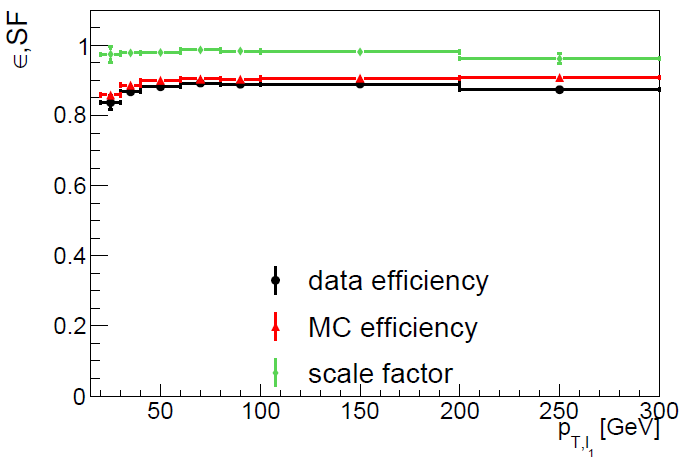
\includegraphics{Chapter1/Figures/Trigger_pt_nosilep.png}}
    \resizebox{0.48 \textwidth}{!}{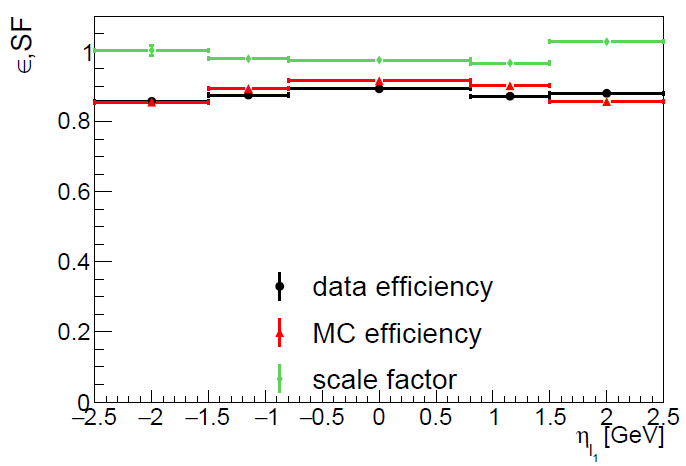
\includegraphics{Chapter1/Figures/Trigger_eta_nosilep.png}}
    \resizebox{0.48 \textwidth}{!}{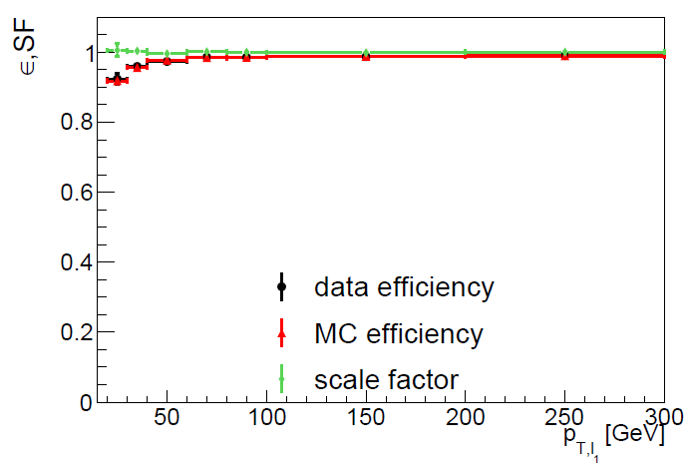
\includegraphics{Chapter1/Figures/Trigger_pt.png}}
    \resizebox{0.48 \textwidth}{!}{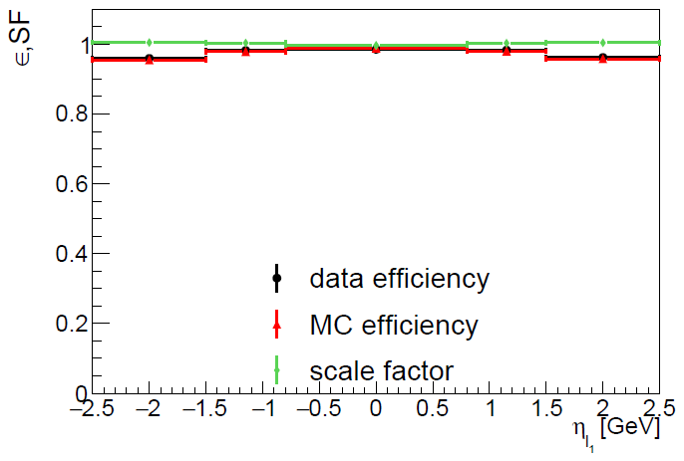
\includegraphics{Chapter1/Figures/Trigger_eta.png}}
      \caption{Efficiencies of the trigger selection in the \emu channel for simulation and data and the corresponding scale factor. The top row shows the efficiency when using dilepton triggers only, while the bottom row shows
      the efficiency for a combination of dilepton and single lepton triggers. The left row shows the efficiency depending on the \pt of the leading lepton. The right column shows the efficiency depending on the $\eta$ of the leading lepton. }  
       \label{fig:TriggerSel}
  \end{center}
\end{figure}


The final trigger selection is a bit more complicated because we aim to take unprescaled triggers with the most relaxed requirements possible.
This results in the trigger selection shown in Table \ref{tab:triggerSel} for each of the three di-lepton channels.
Double counting events is prevented by explicitly requiring triggers on their respective dataset, but vetoing them on the other datasets.

 \begin{table}[hbt]
    \centering
    \caption{The trigger selection that is applied on data. It can differ between the different run periods because of changing prescales.}
    \label{tab:triggerSel}
     \begin{tabular}
            {c|c|c}
            channel & run & trigger \\
            \hline
             \mumu & B-G & HLT\_Mu17\_TrkIsoVVL\_Mu8\_TrkIsoVVL \\
              & B-G & HLT\_Mu17\_TrkIsoVVL\_TkMu8\_TrkIsoVVL \\
              & H & HLT\_Mu17\_TrkIsoVVL\_Mu8\_TrkIsoVVL\_DZ \\
              & H & HLT\_Mu17\_TrkIsoVVL\_TkMu8\_TrkIsoVVL\_DZ \\
              & B-H & HLT\_IsoMu24 \\
              & B-H & HLT\_IsoTkMu24 \\
            \hline
             \ee &  B-H & HLT\_Ele23\_Ele12\_CaloIdL\_TrackIdL\_IsoVL\_DZ \\
              &  B-H & HLT\_Ele27\_WPTight\_Gsf \\
            \hline
             \empm & B-G & HLT\_Mu23\_TrkIsoVVL\_Ele12\_CaloIdL\_TrackIdL\_IsoVL \\
              & B-G & HLT\_Mu8\_TrkIsoVVL\_Ele23\_CaloIdL\_TrackIdL\_IsoVL \\
              & H & HLT\_Mu23\_TrkIsoVVL\_Ele12\_CaloIdL\_TrackIdL\_IsoVL\_DZ \\
              & H & HLT\_Mu8\_TrkIsoVVL\_Ele23\_CaloIdL\_TrackIdL\_IsoVL\_DZ \\
              & B-H & HLT\_Ele27\_WPTight\_Gsf \\
              & B-H & HLT\_IsoMu24 \\
              & B-H & HLT\_IsoTkMu24 \\
    \end{tabular}
\end{table}







%********************************** %Second Section  *************************************
\section{Method: Independent Triggers} %Section - 1.2
\label{sec:TriggerMetMethod}

In this analysis the trigger efficiency is mainly measured using a dataset taken with an orthogonal trigger selection.
In general this allows to measure the trigger efficiency without bias with the same method in data and simulation independently 
of each other. It is important that these independent triggers are indeed as independent from the dilepton triggers as possible
and for simplicity they should also be unprescaled in the full run range.

Here triggers based on missing transverse energy (\ETm) are used. They are especially usefull for a \ttbar analysis, 
as dileptonic \ttbar events should produce \ETm due to the two neutrinos. This allows to measure the trigger efficiency for data
in an event sample which at least contains \ttbar events. The efficiency in simulation can be measured on a sample of \ttbar events.

The trigger efficiency is then measured according to the formula given in Equation \ref{eq:TriggerEff}, where $N$ denotes the number of 
events fullfilling the given requirements.

\begin{equation}
\varepsilon_{trig} = \frac{N(\mathrm{Offline Selection + \ETm \; Trigger + Measured Trigger})}{N(\mathrm{Offline Selection + \ETm \; Trigger})}
\label{eq:TriggerEff}
\end{equation}

The efficiency is measured for each event, consequently the resulting scale factors to be applied on simulation to correct to data are applied per event as well.
This is especially useful if a combination of multiple triggers is used in the selection.

The statistical uncertainty is calculated assuming a binomial distribution using the Clopper-Pearson method \todo{cit PDG}. It offers at least nominal coverage 
of the given confidence level and preesents the conservative option to estimate these uncertainties. 

Results for efficiencies and scale factors for the \ee, \mumu and \emu channel are shown in figures \ref{fig:MET_ee},\ref{fig:MET_mumu} and \ref{fig:MET_emu} respectively.

\begin{figure}[htbp!]
  \begin{center}
    \resizebox{0.48 \textwidth}{!}{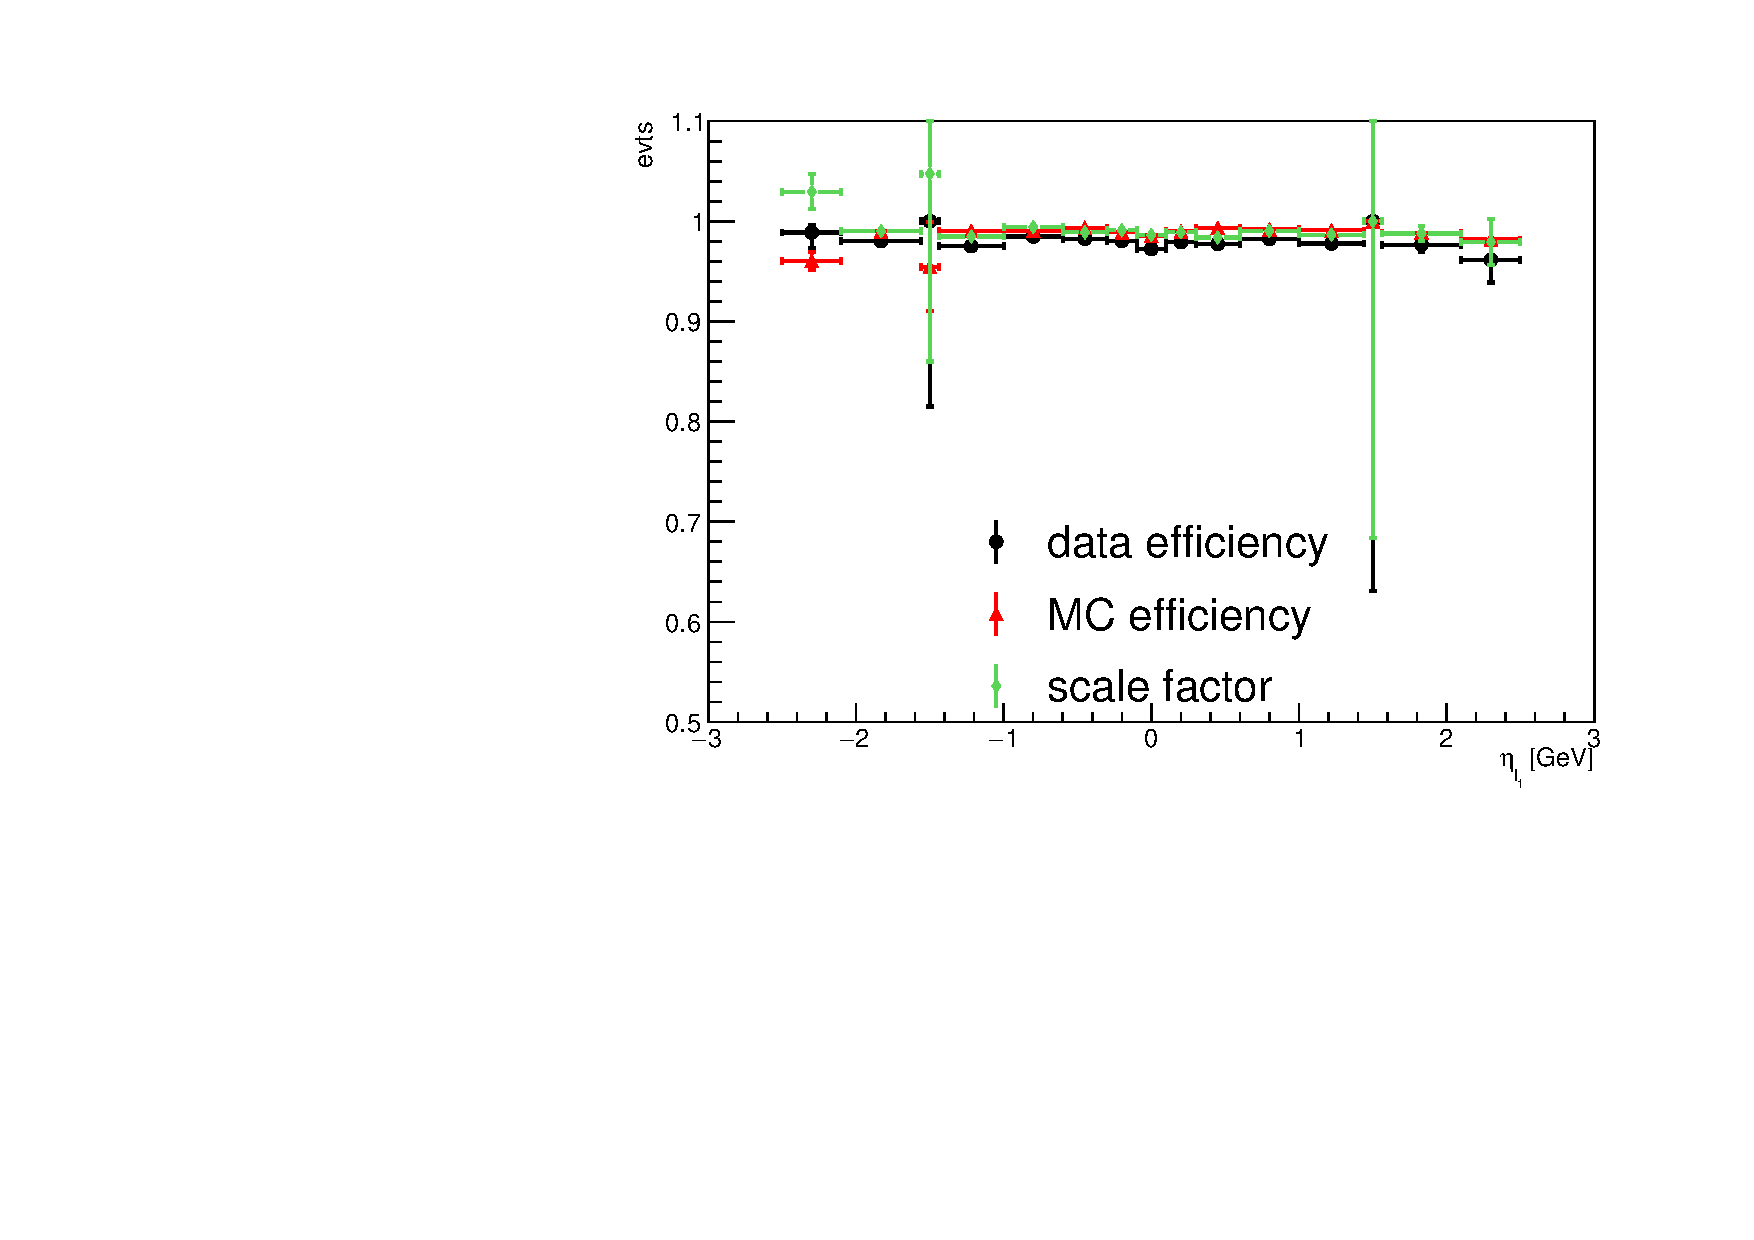
\includegraphics{Chapter1/Figures/MET/ee/leading_eta}}
    \resizebox{0.48 \textwidth}{!}{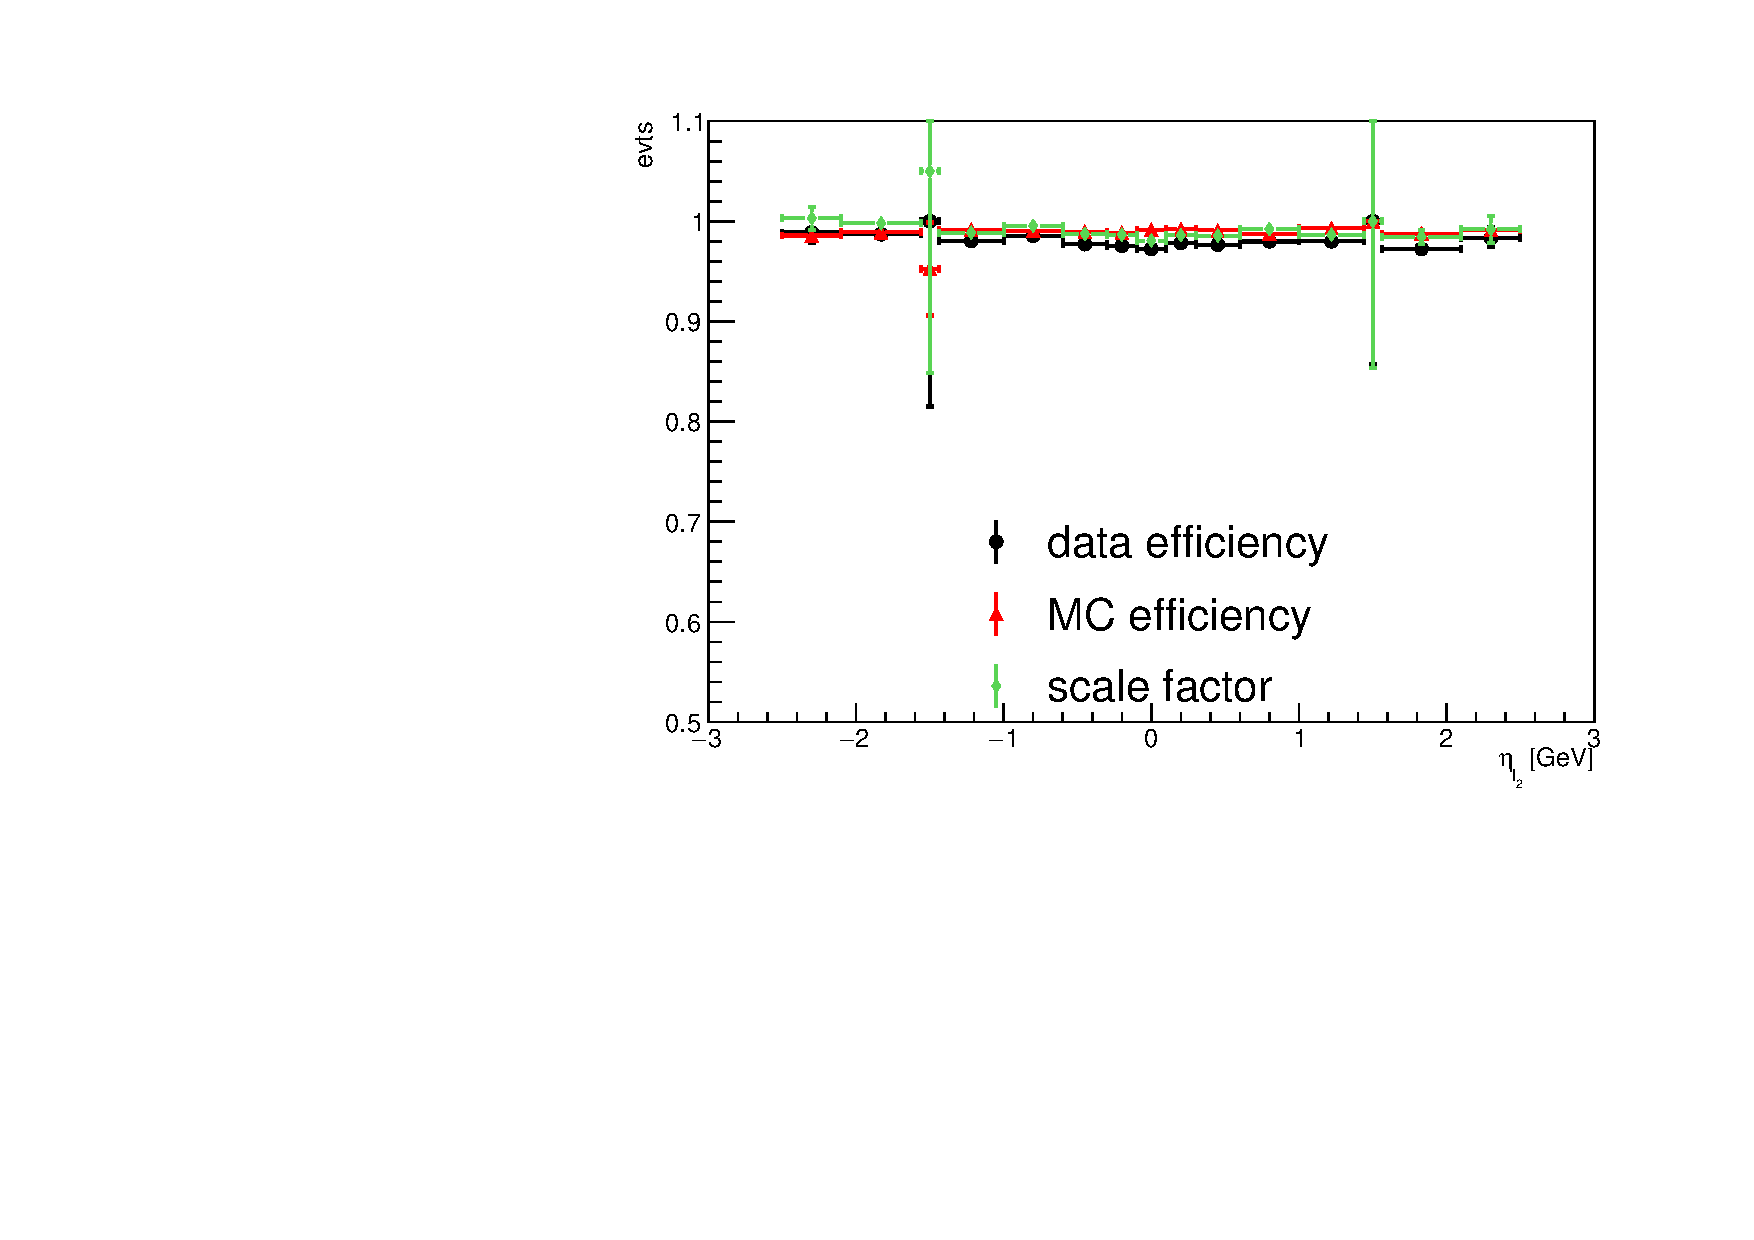
\includegraphics{Chapter1/Figures/MET/ee/seleading_eta}}
    \resizebox{0.48 \textwidth}{!}{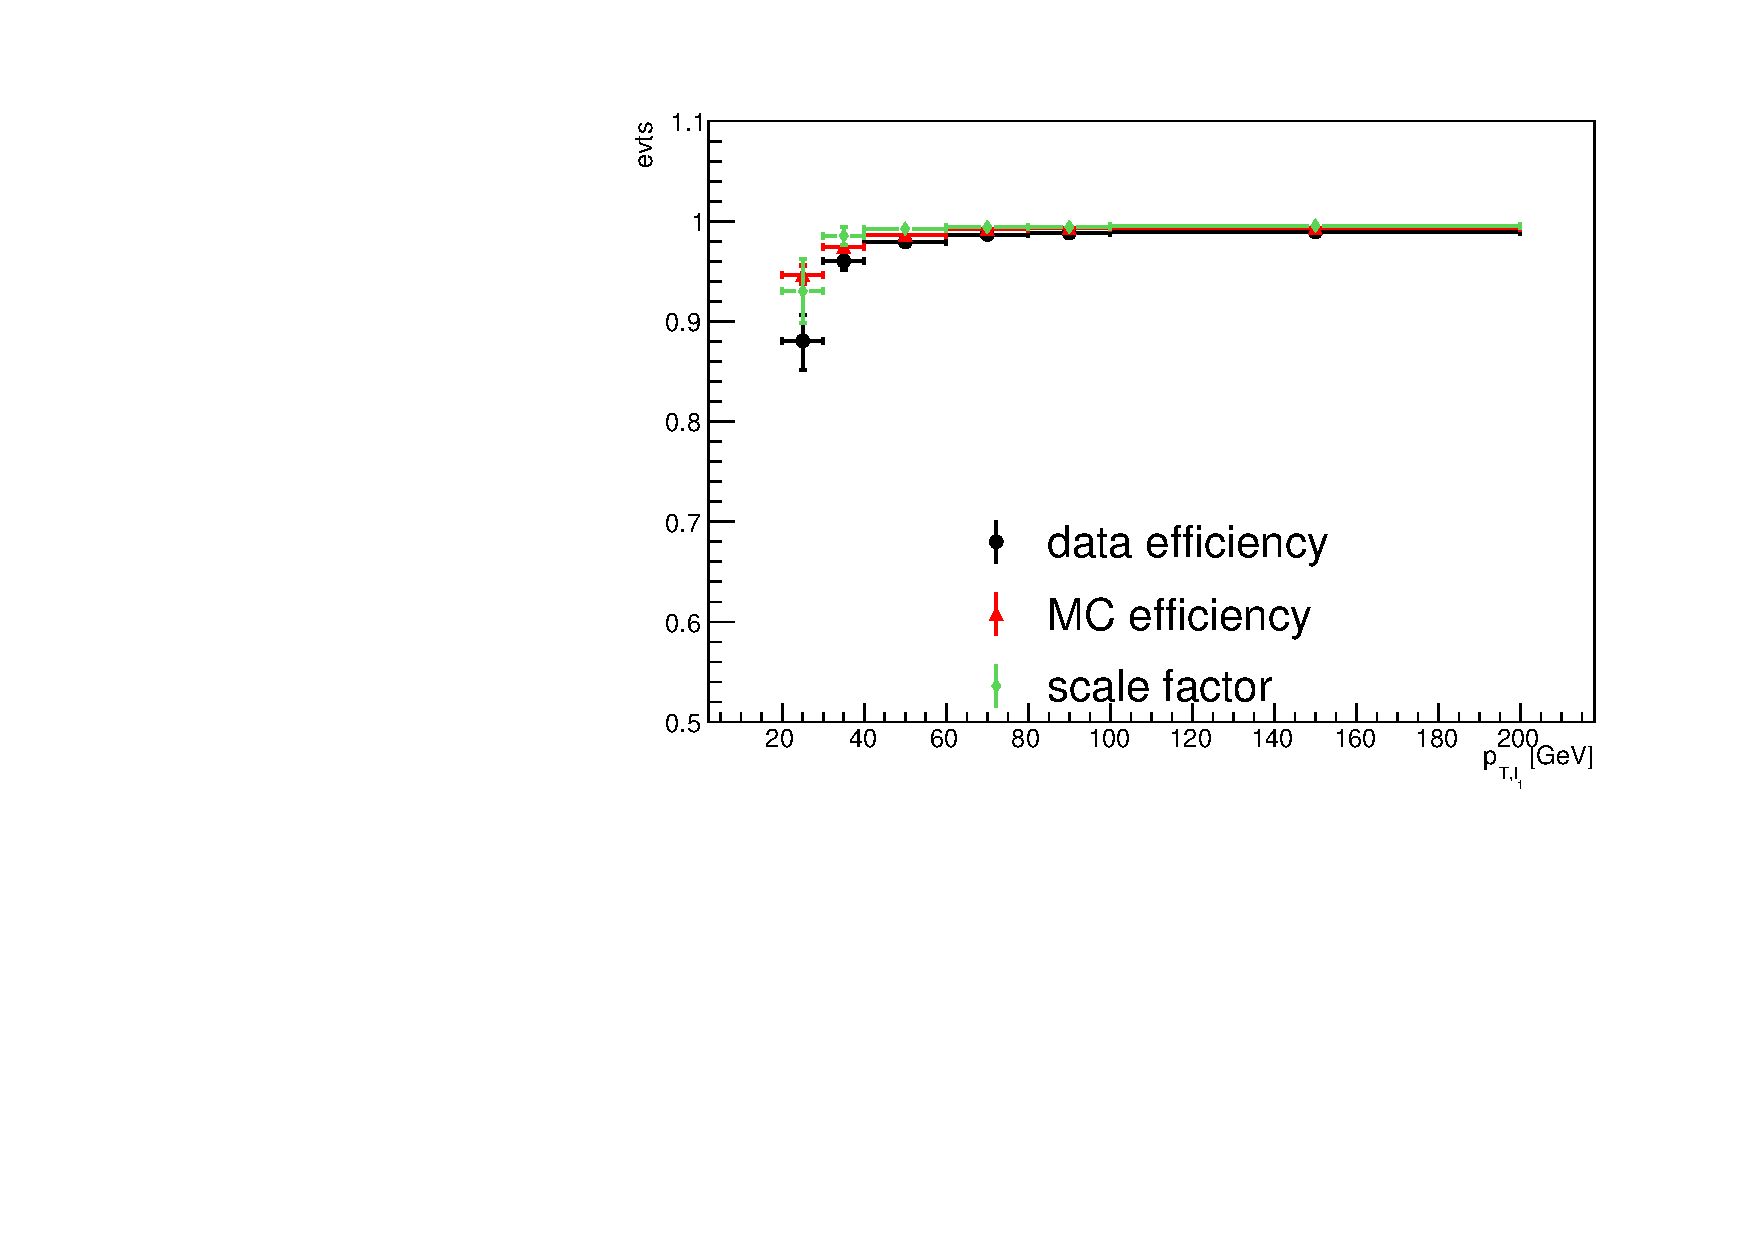
\includegraphics{Chapter1/Figures/MET/ee/leading_pt}}
    \resizebox{0.48 \textwidth}{!}{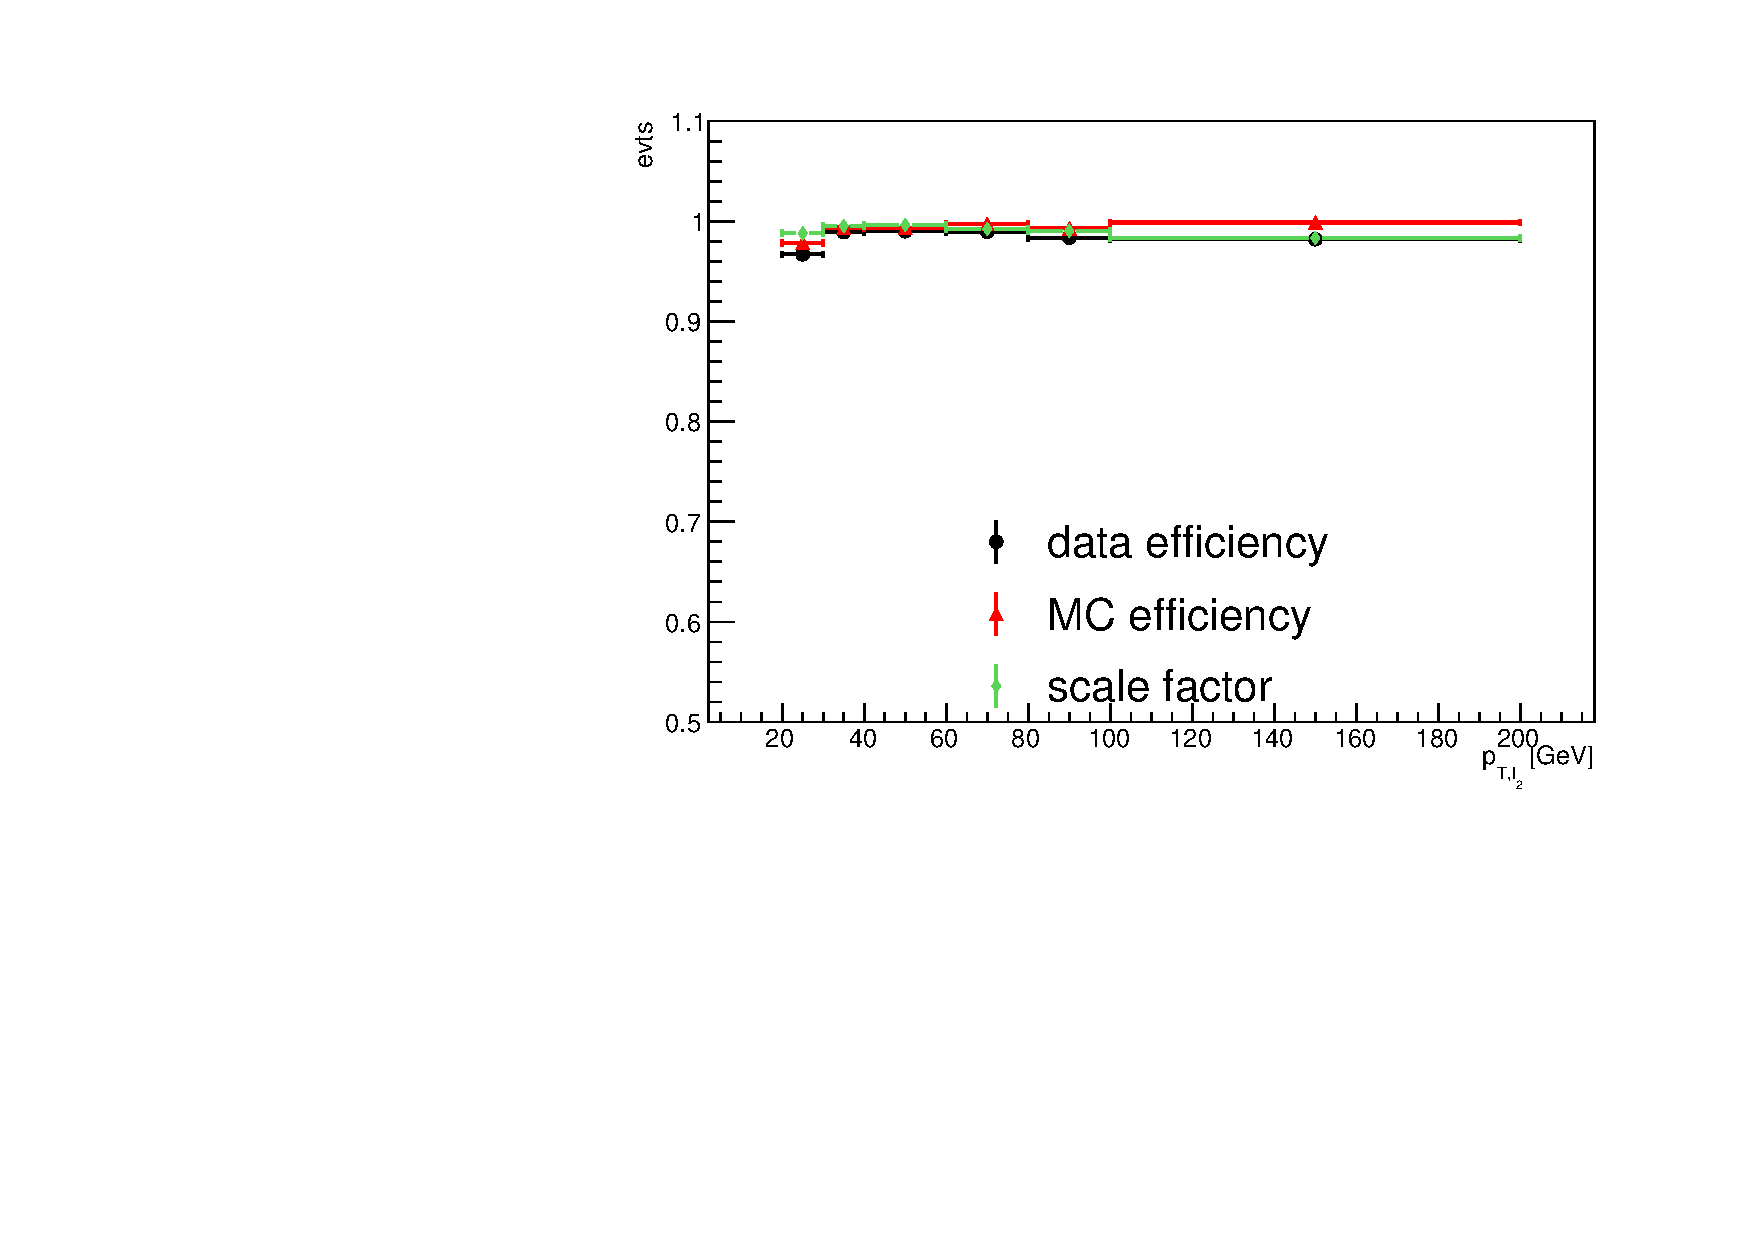
\includegraphics{Chapter1/Figures/MET/ee/seleading_pt}}
    \resizebox{0.48 \textwidth}{!}{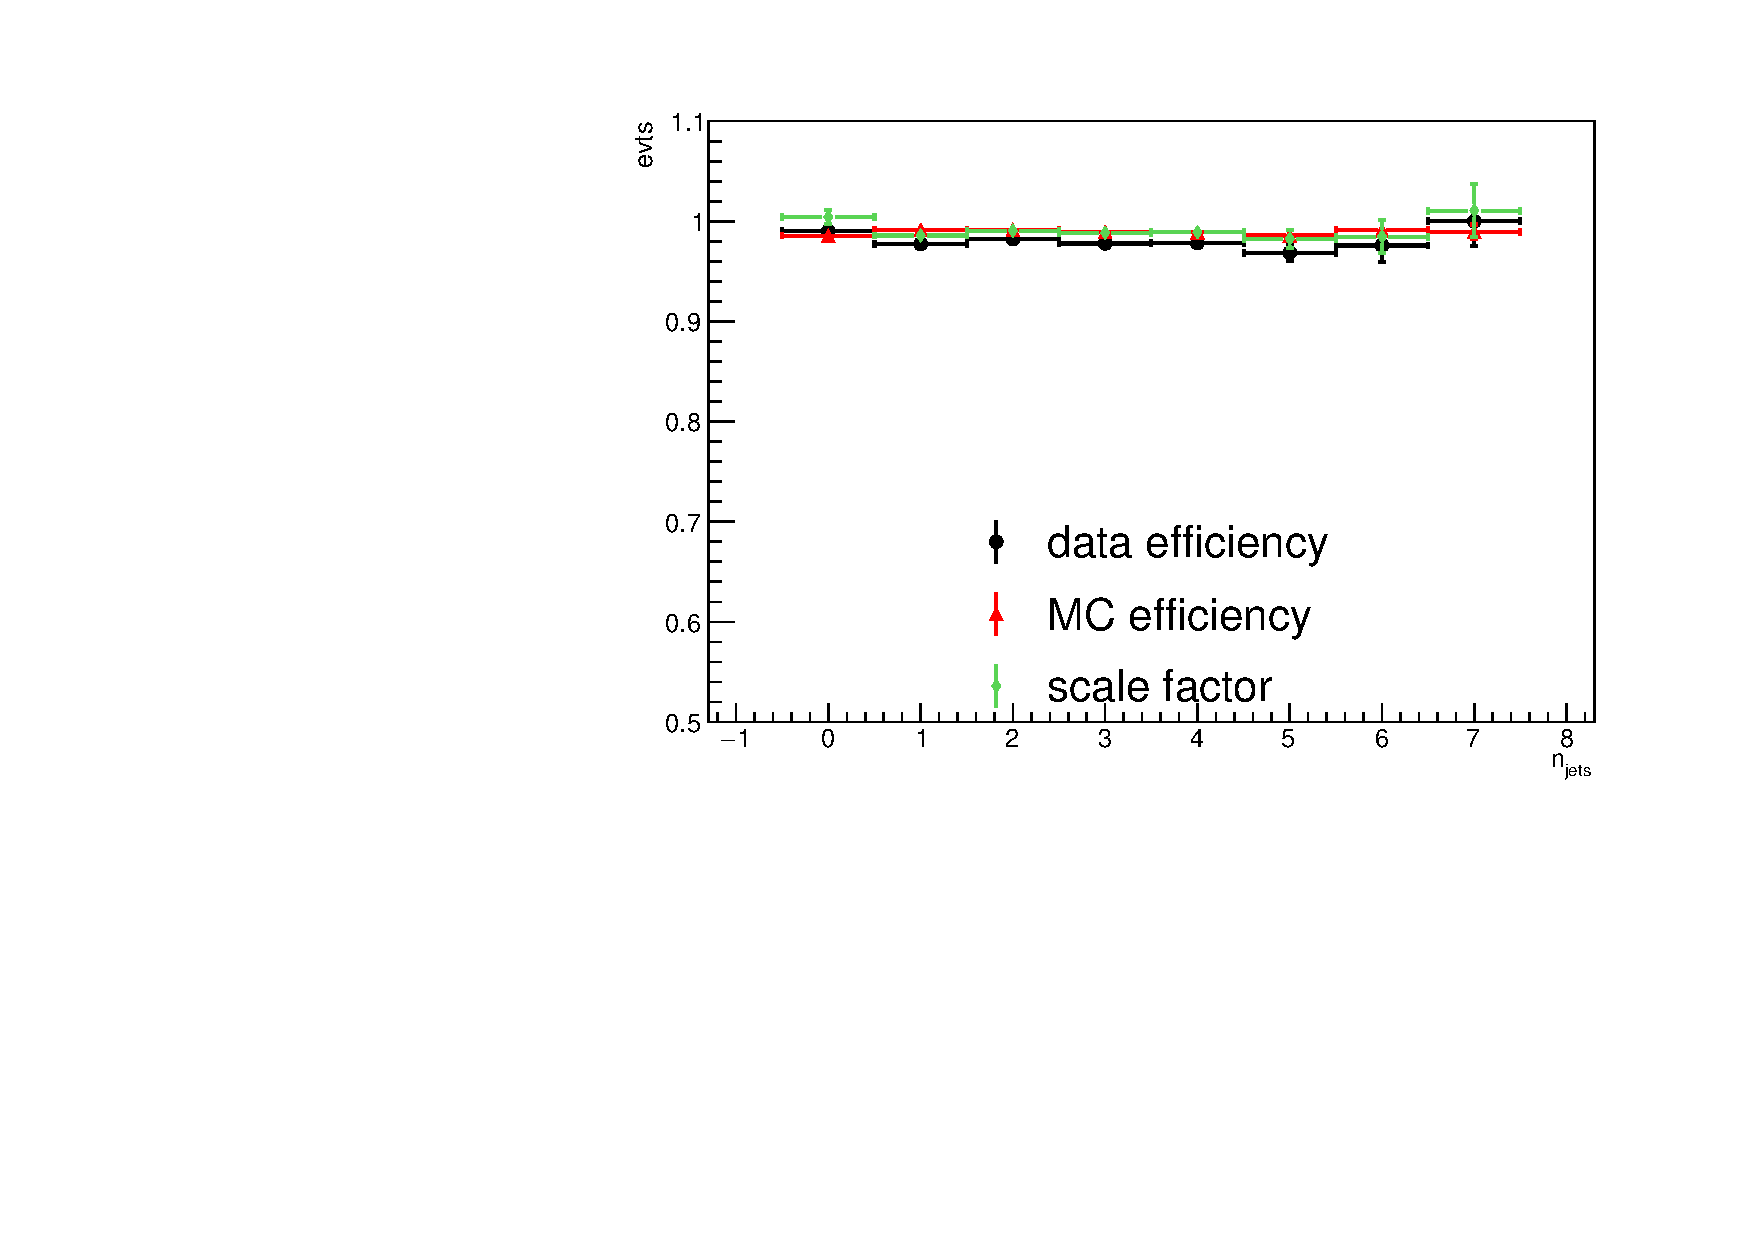
\includegraphics{Chapter1/Figures/MET/ee/jet_multi}}
    \resizebox{0.48 \textwidth}{!}{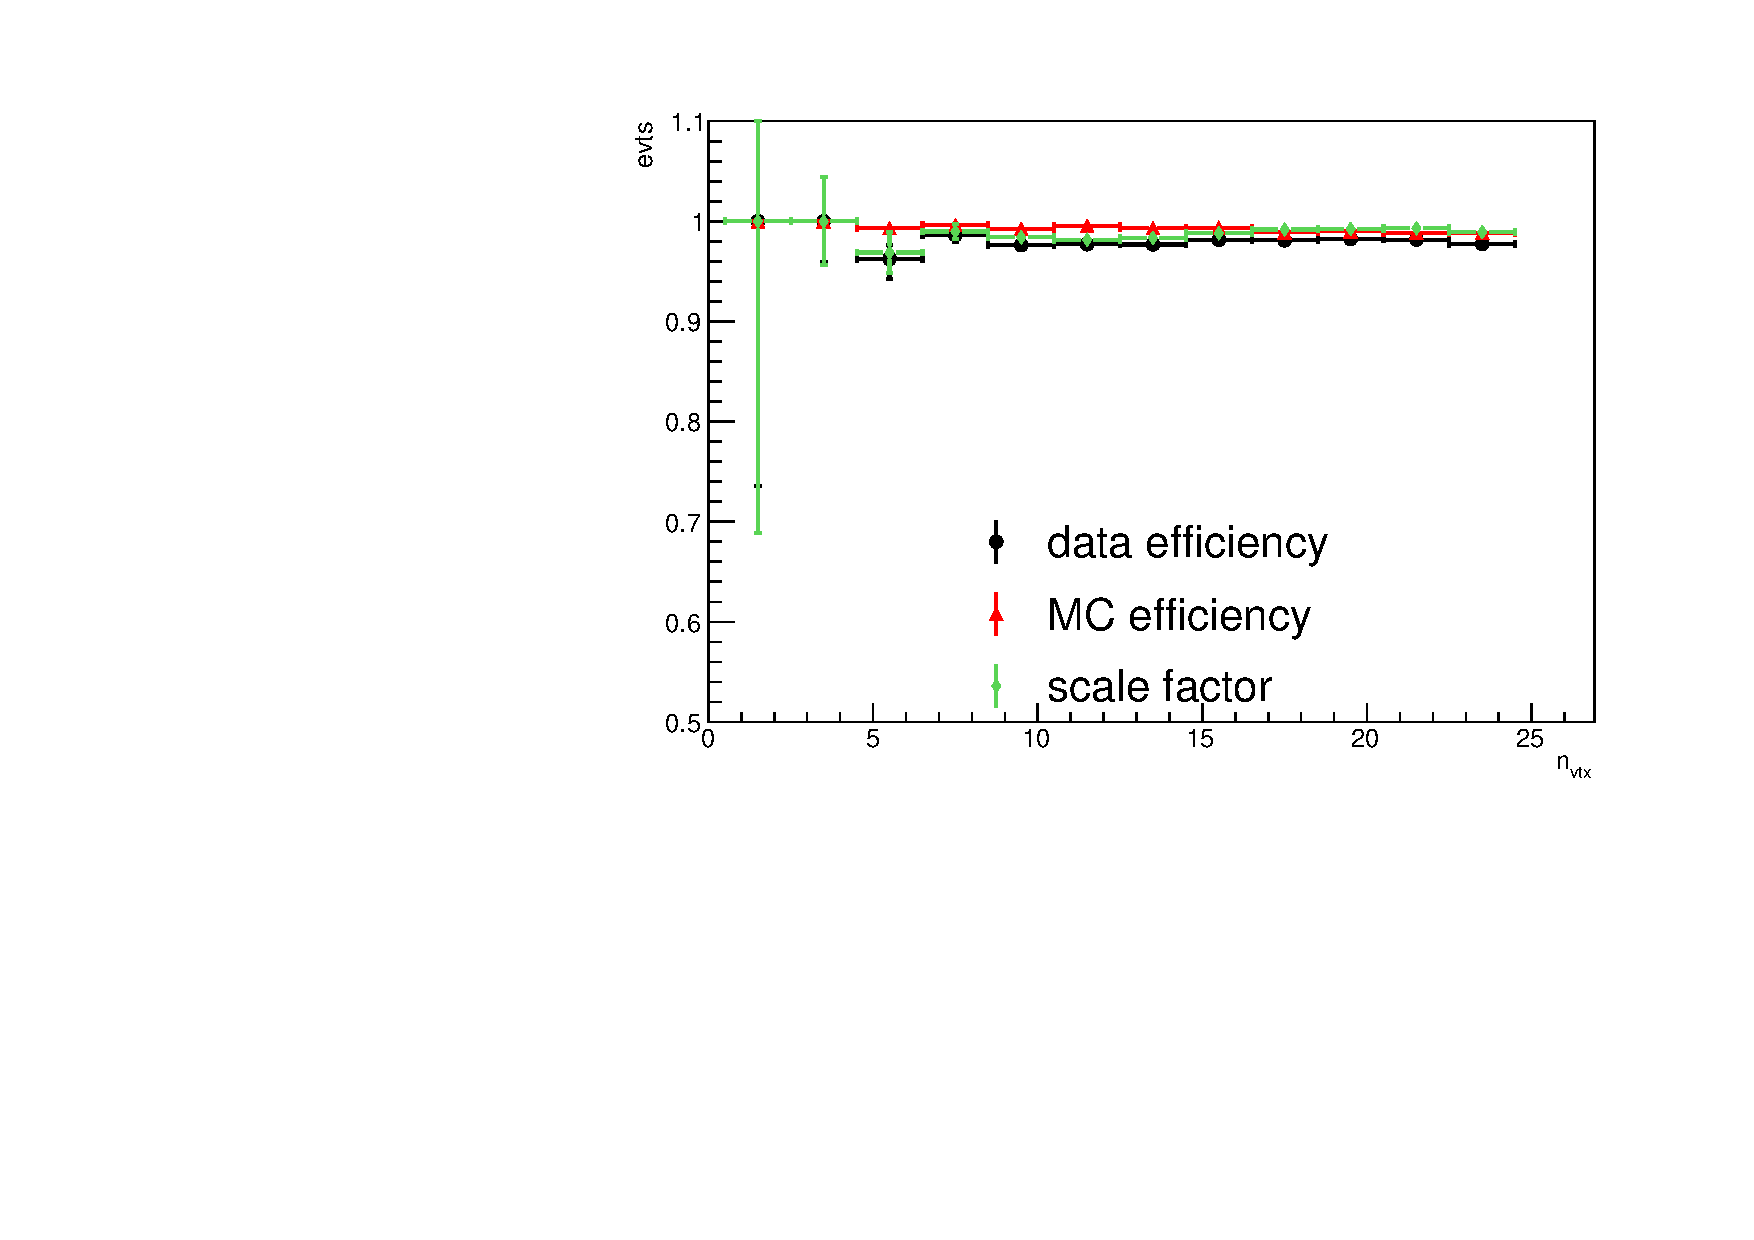
\includegraphics{Chapter1/Figures/MET/ee/vertex_multi}}  
      \caption{Efficiencies of the trigger selection in the \ee channel for simulation and data and the corresponding scale factor. The top row shows the efficiency depending on $\eta$ of the leading (left) and trailing (right) lepton. The middle row shows the effciency \pt of the leading (left) and trailing (right) lepton. The bottom rwo shows the efficiency depending on the jet multiplicity on the left and the vertex multiplicity on the right.
       The error bars denote statistical uncertainties. }  
      
    \label{fig:MET_ee}
  \end{center}
\end{figure}

\begin{figure}[htbp!]
  \begin{center}
    \resizebox{0.48 \textwidth}{!}{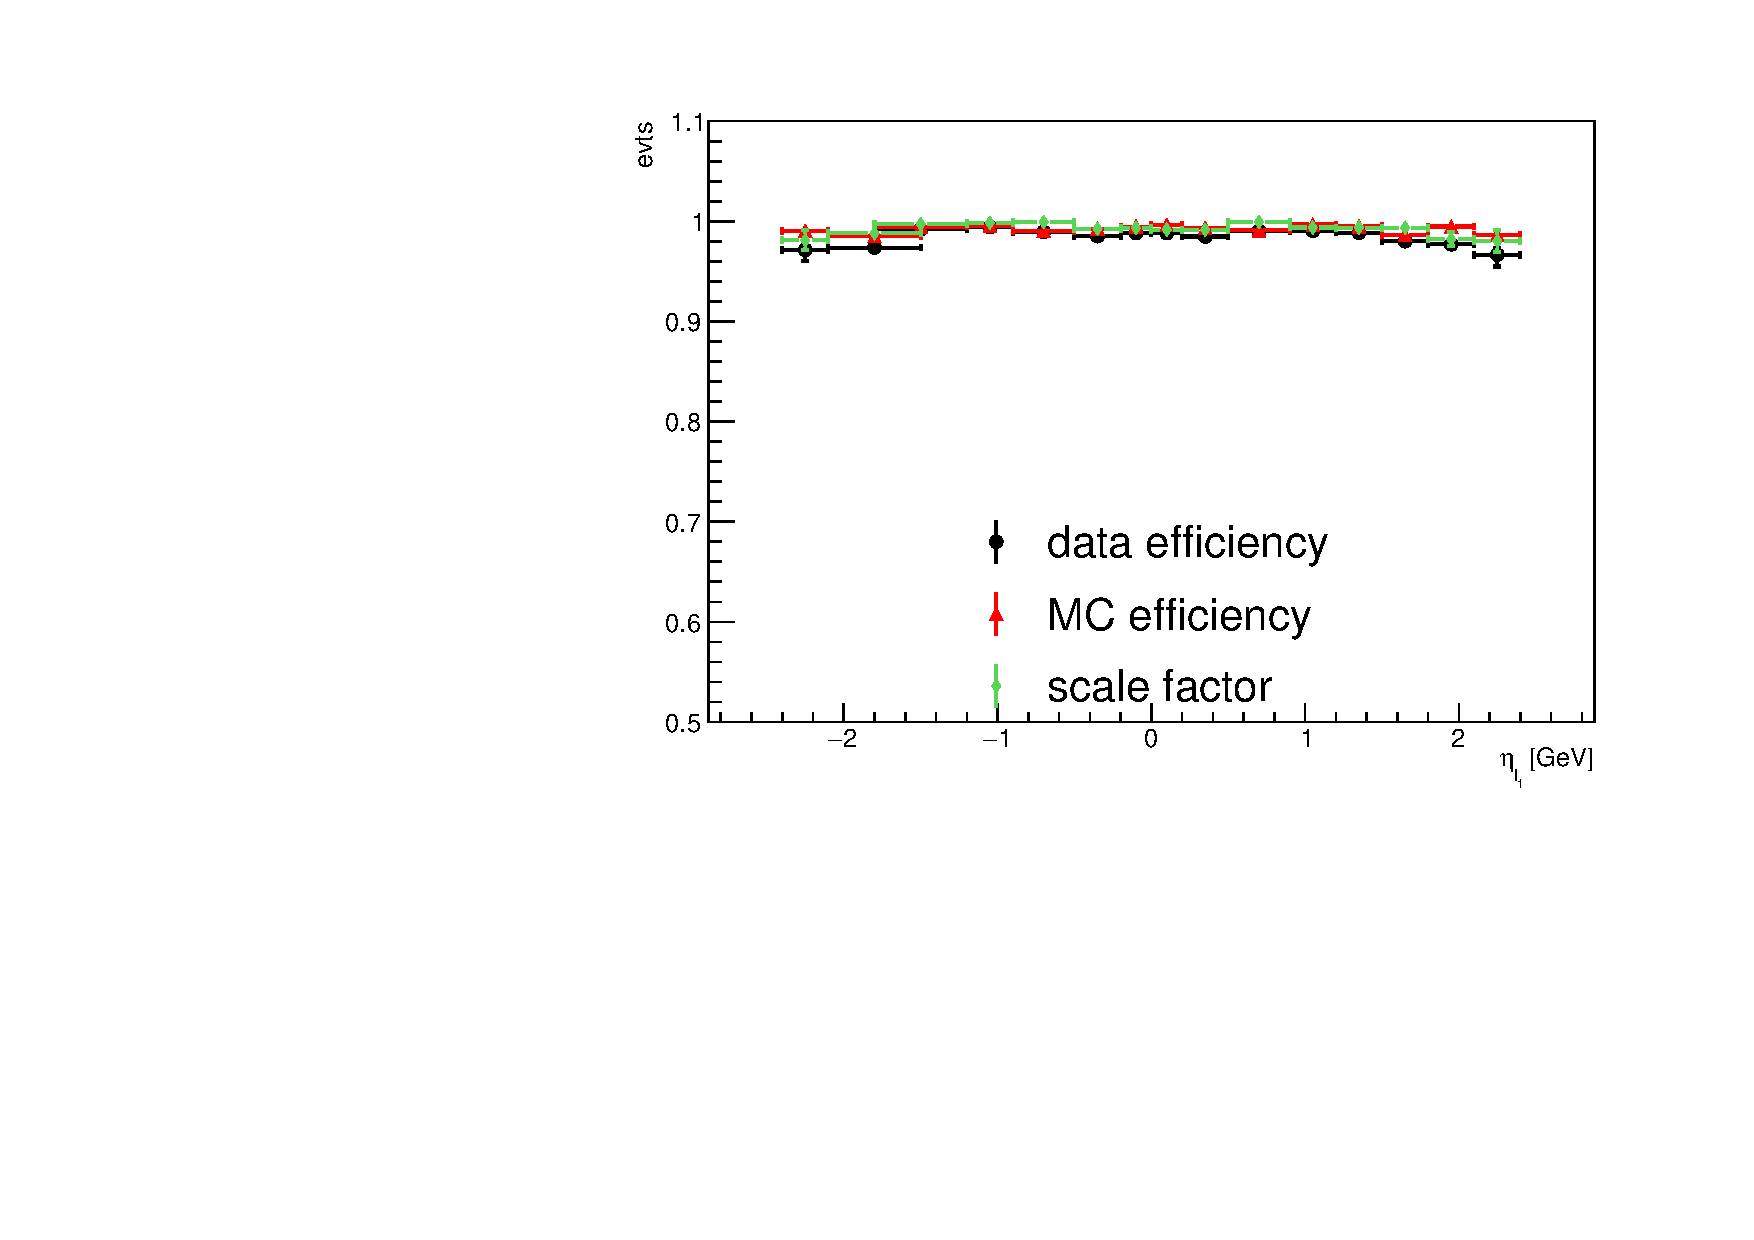
\includegraphics{Chapter1/Figures/MET/mumu/leading_eta}}
    \resizebox{0.48 \textwidth}{!}{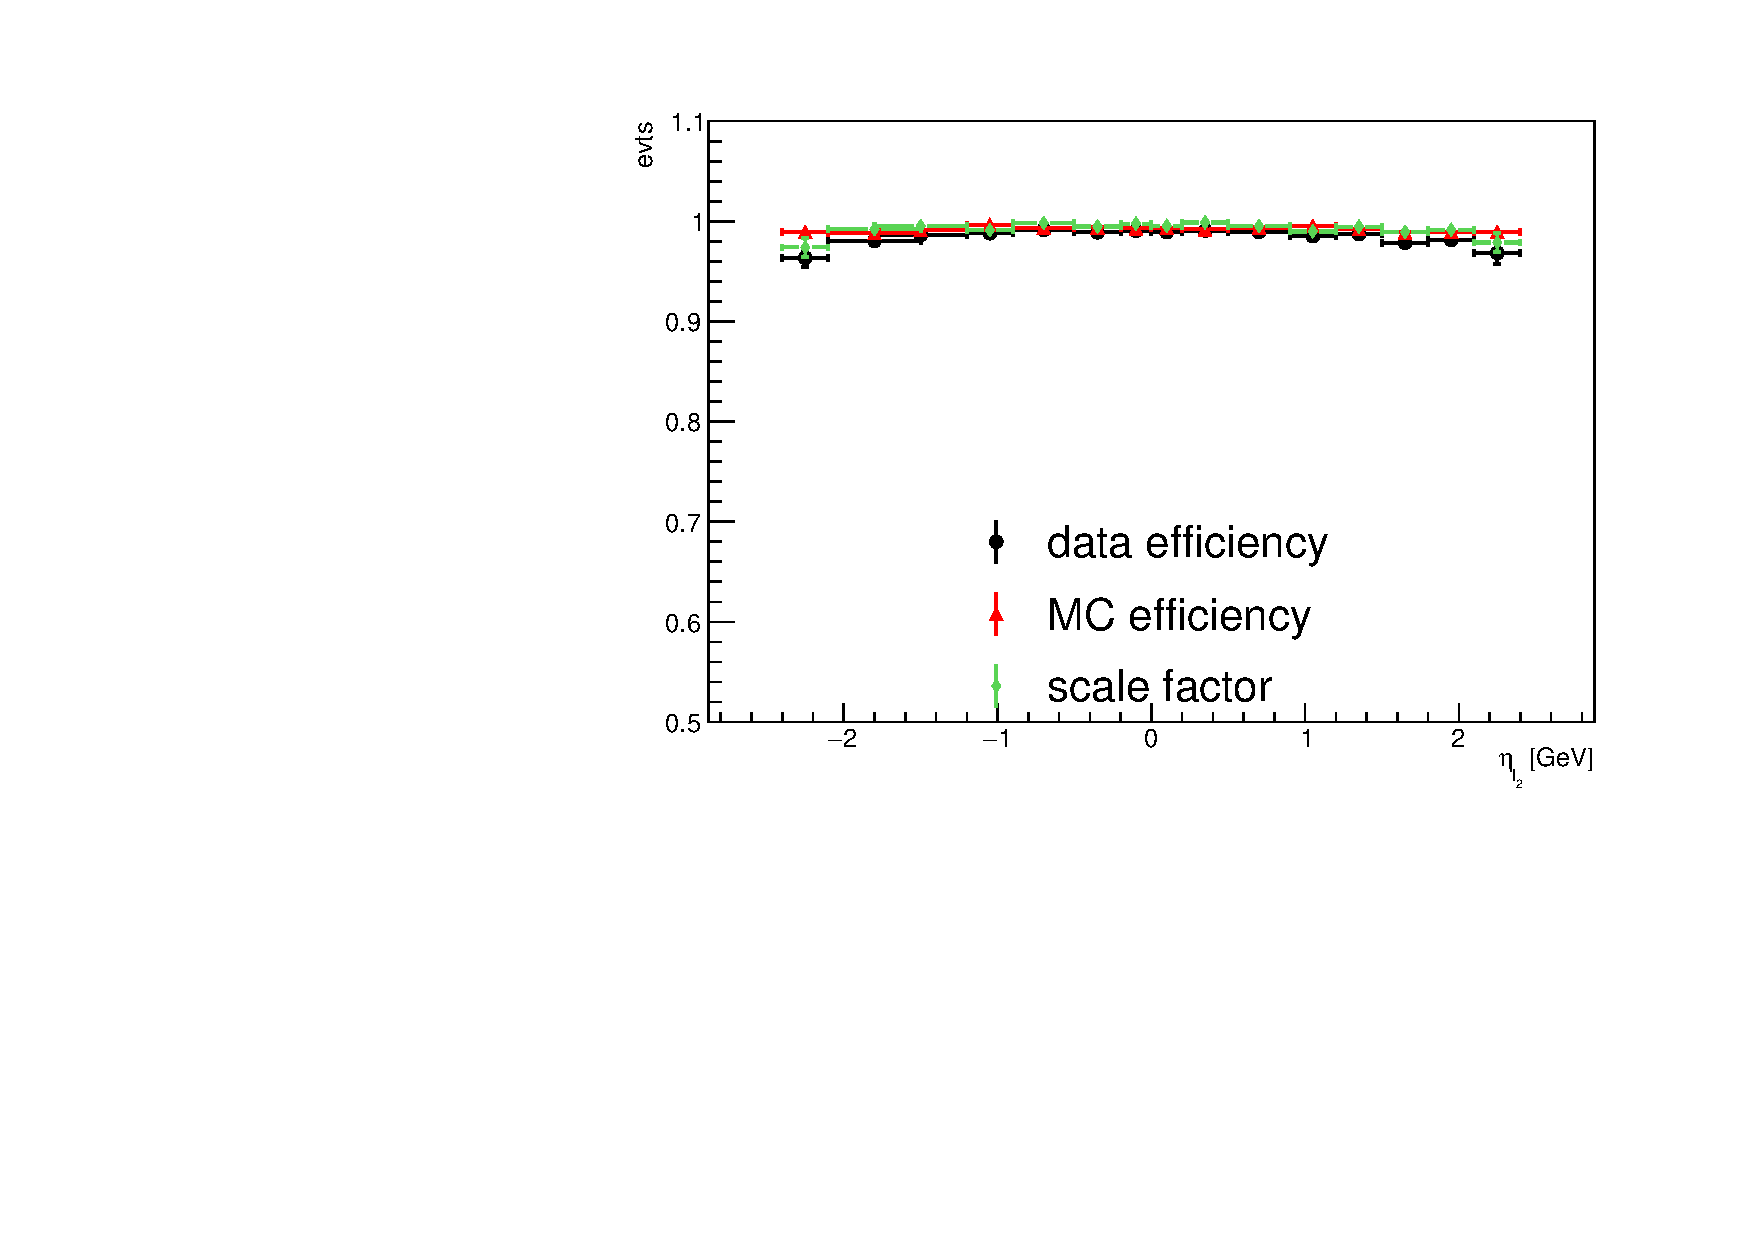
\includegraphics{Chapter1/Figures/MET/mumu/seleading_eta}}
    \resizebox{0.48 \textwidth}{!}{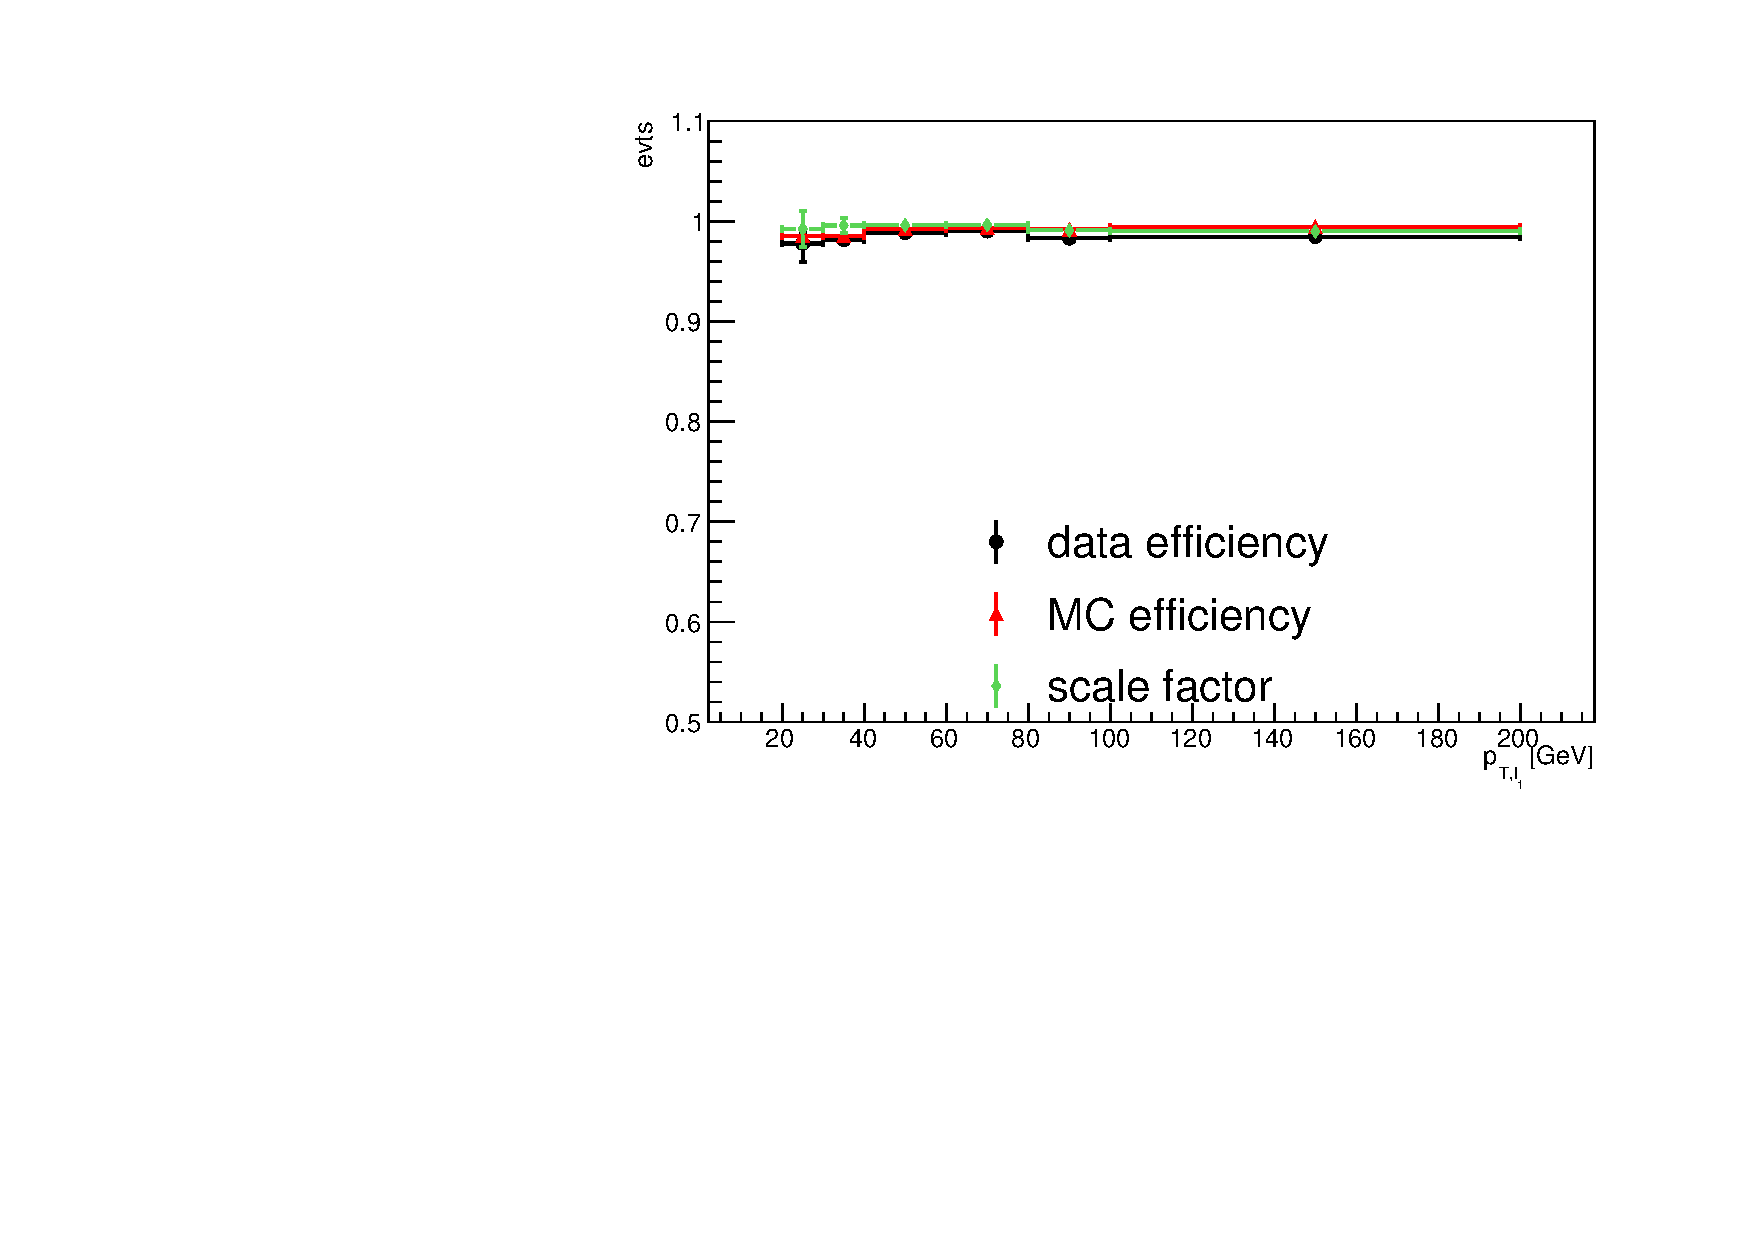
\includegraphics{Chapter1/Figures/MET/mumu/leading_pt}}
    \resizebox{0.48 \textwidth}{!}{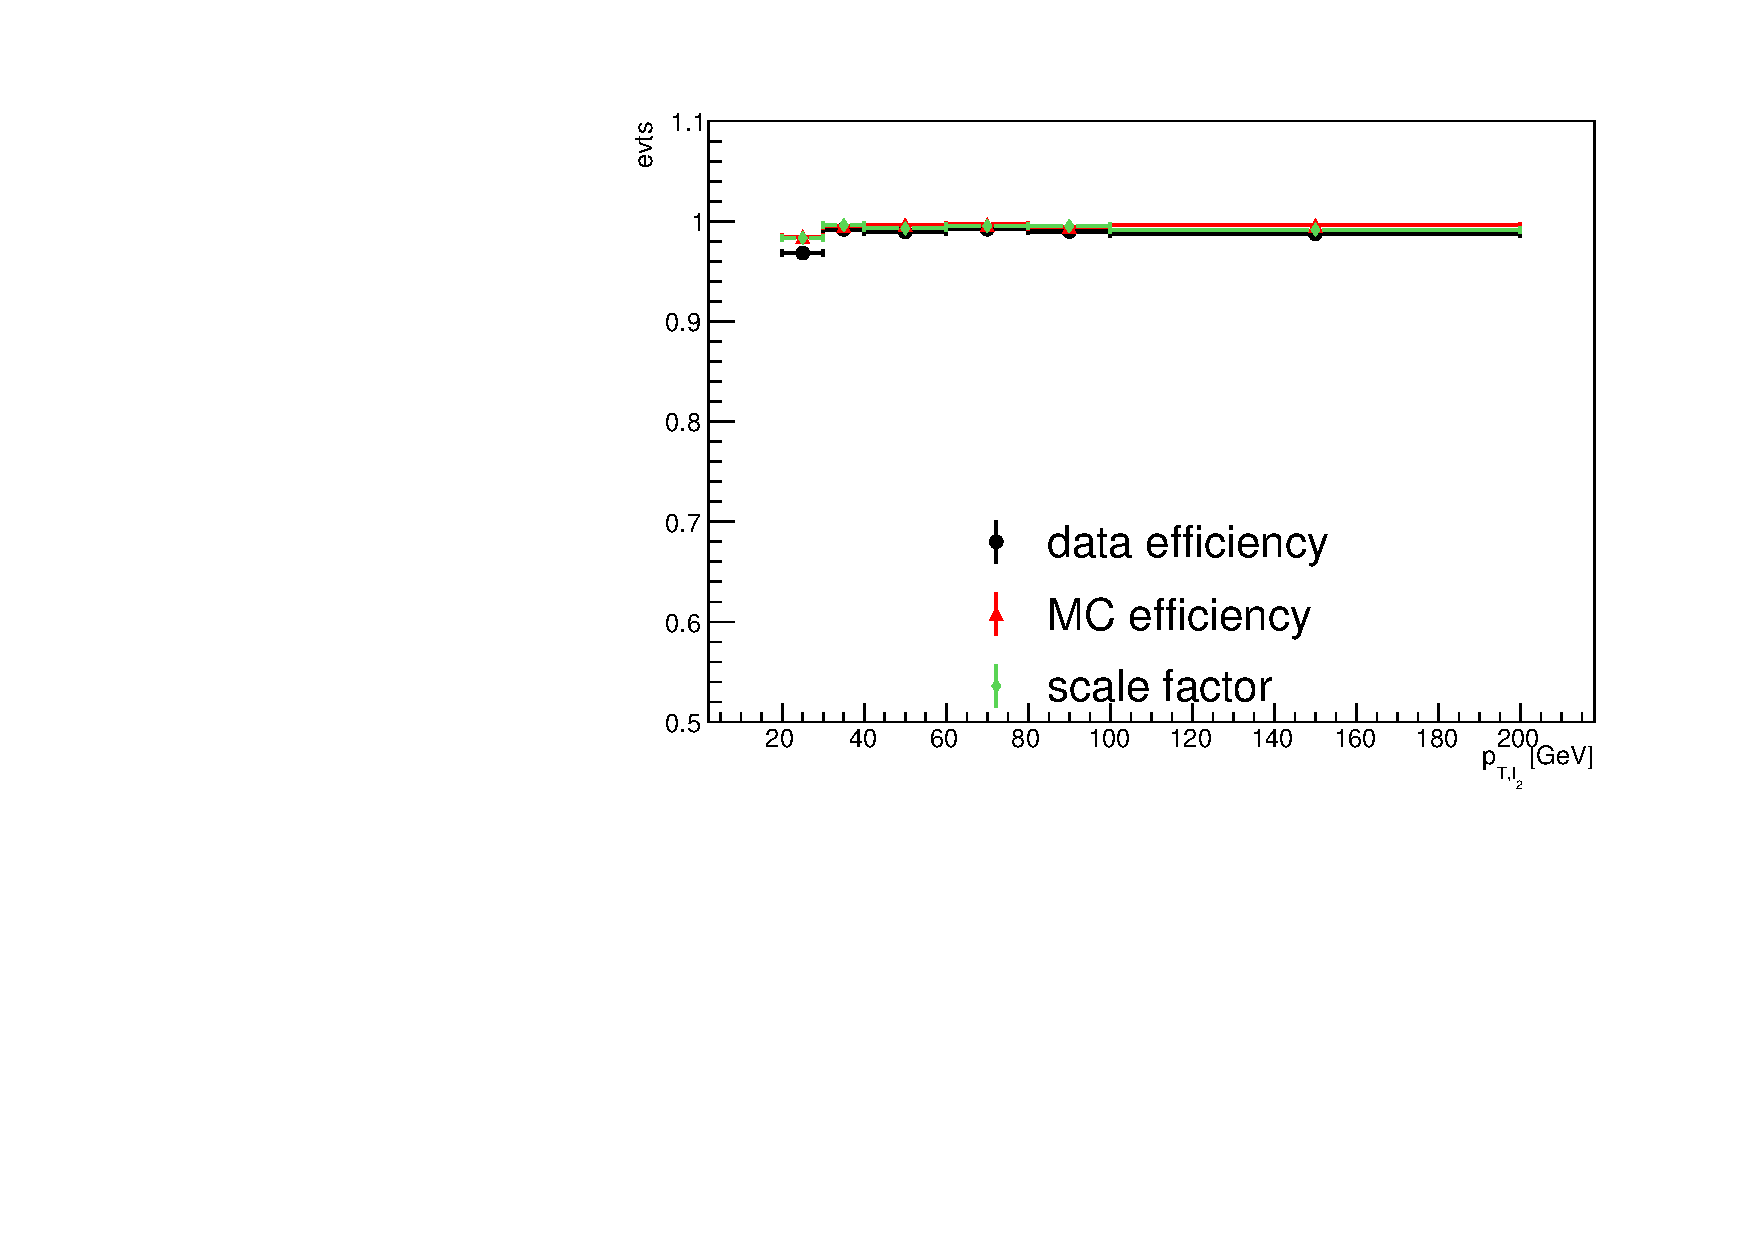
\includegraphics{Chapter1/Figures/MET/mumu/seleading_pt}}
    \resizebox{0.48 \textwidth}{!}{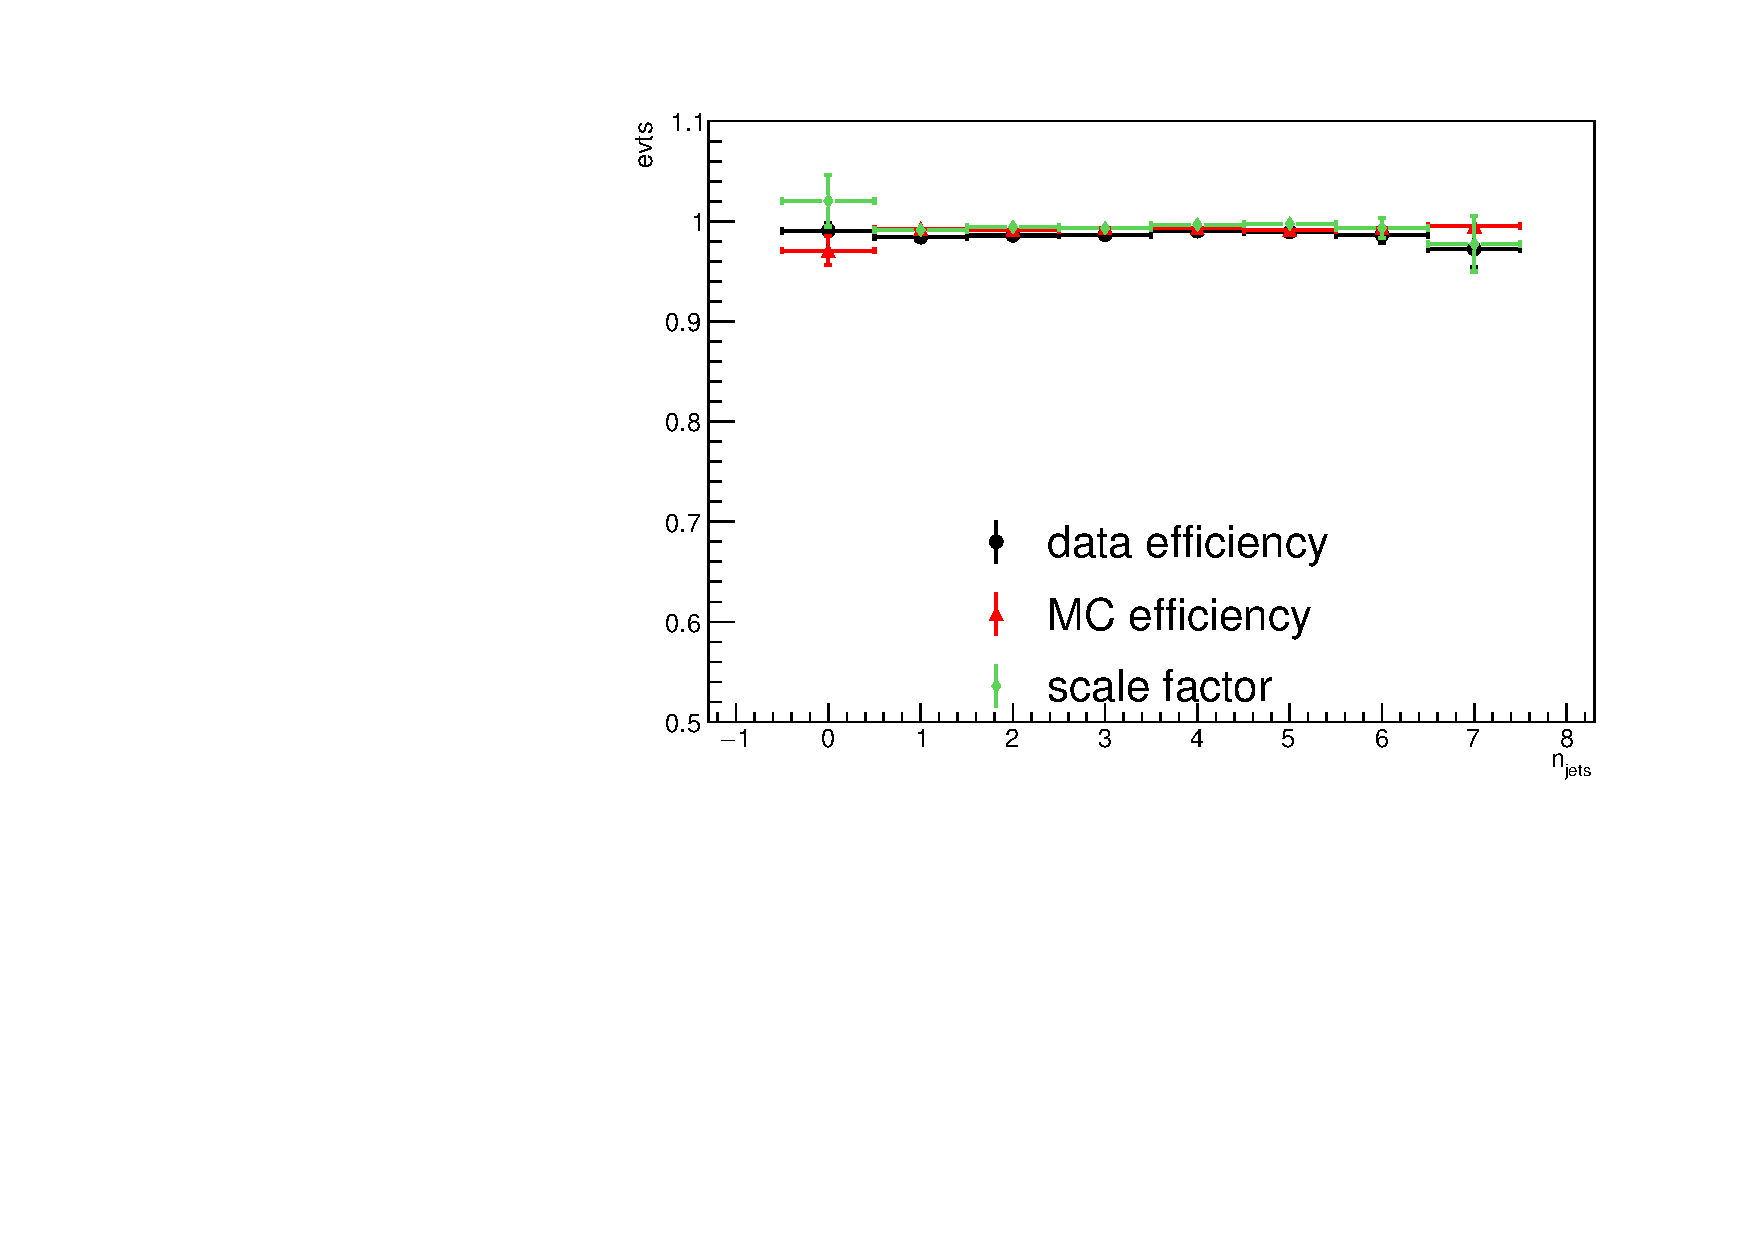
\includegraphics{Chapter1/Figures/MET/mumu/jet_multi}}
    \resizebox{0.48 \textwidth}{!}{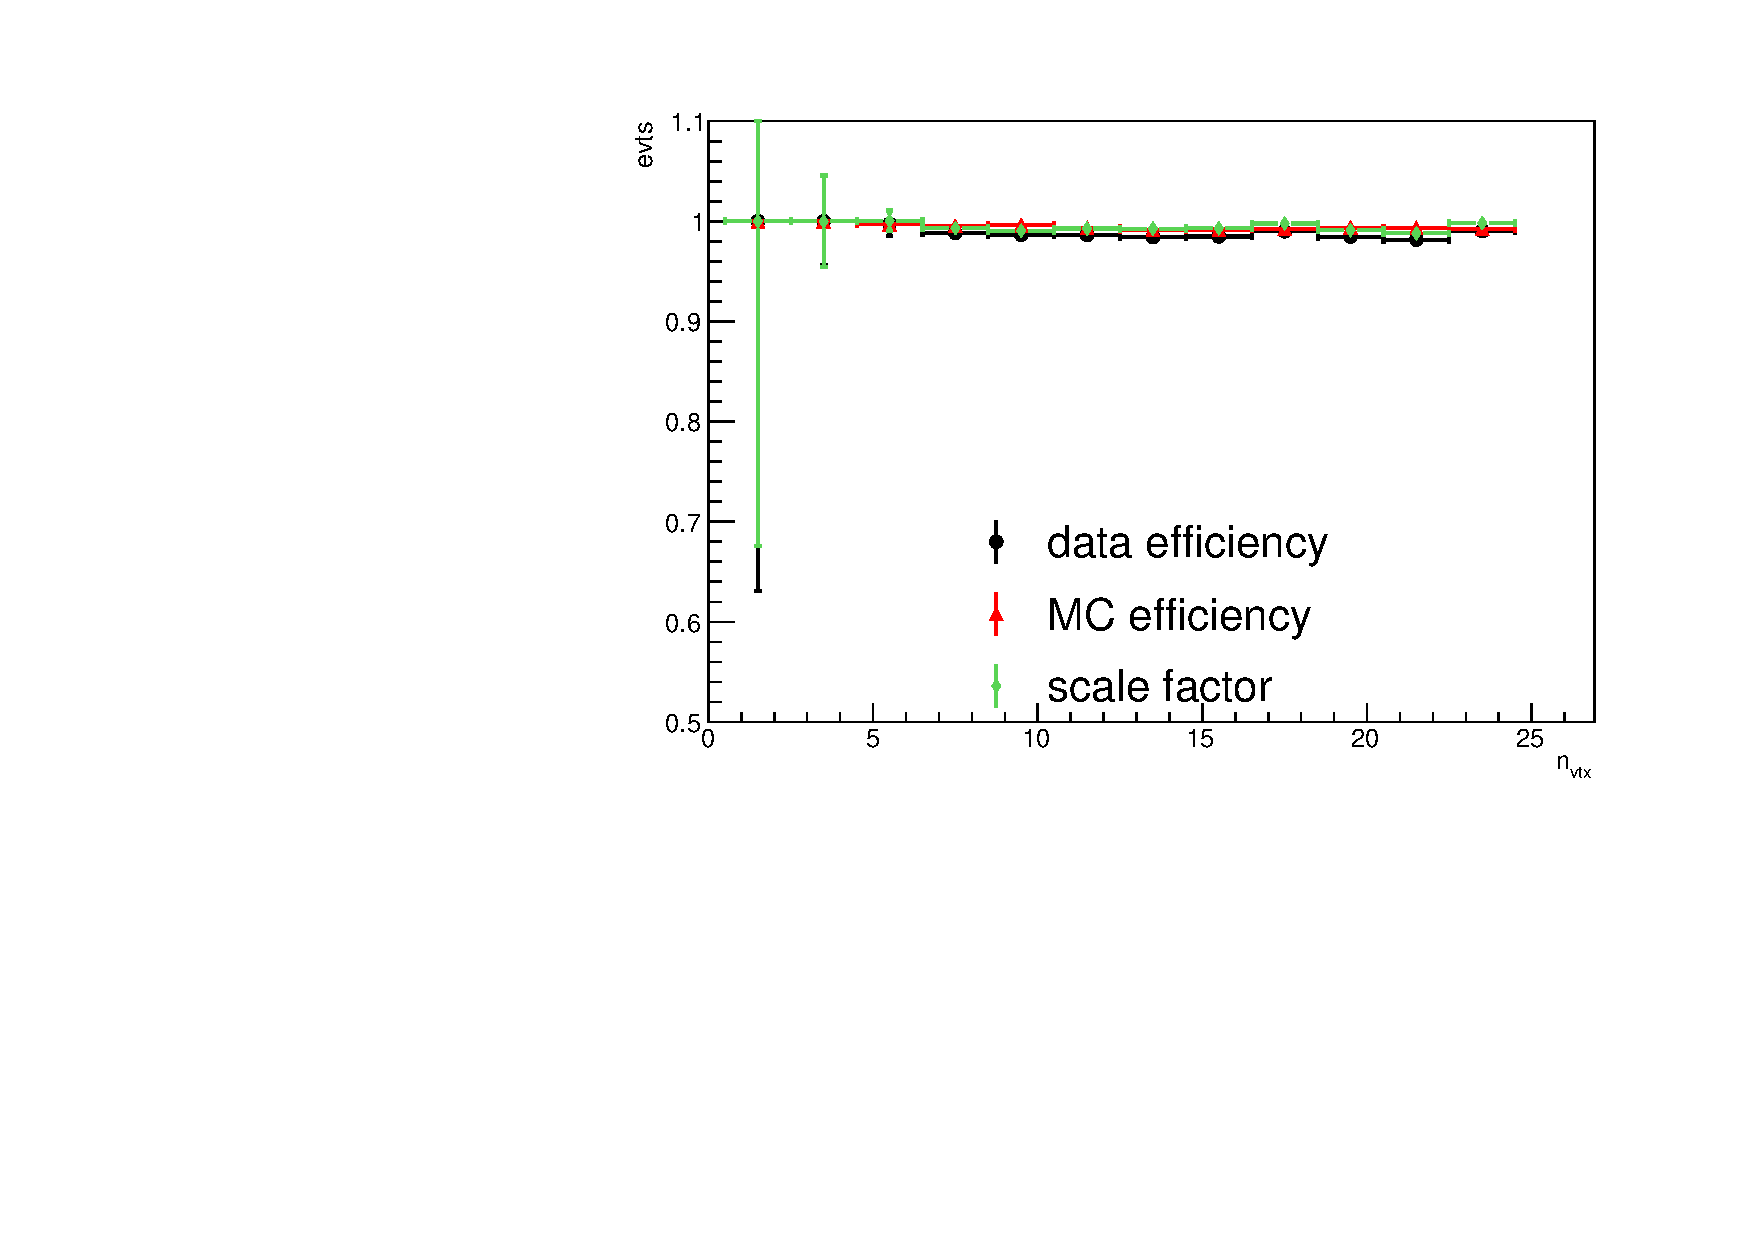
\includegraphics{Chapter1/Figures/MET/mumu/vertex_multi}}  
      \caption{Efficiencies of the trigger selection in the \mumu channel for simulation and data and the corresponding scale factor. The top row shows the efficiency depending on $\eta$ of the leading (left) and trailing (right) lepton. The middle row shows the effciency \pt of the leading (left) and trailing (right) lepton. The bottom rwo shows the efficiency depending on the jet multiplicity on the left and the vertex multiplicity on the right.
      The error bars denote statistical uncertainties. }  
      
    \label{fig:MET_mumu}
  \end{center}
\end{figure}

\begin{figure}[htbp!]
  \begin{center}
    \resizebox{0.48 \textwidth}{!}{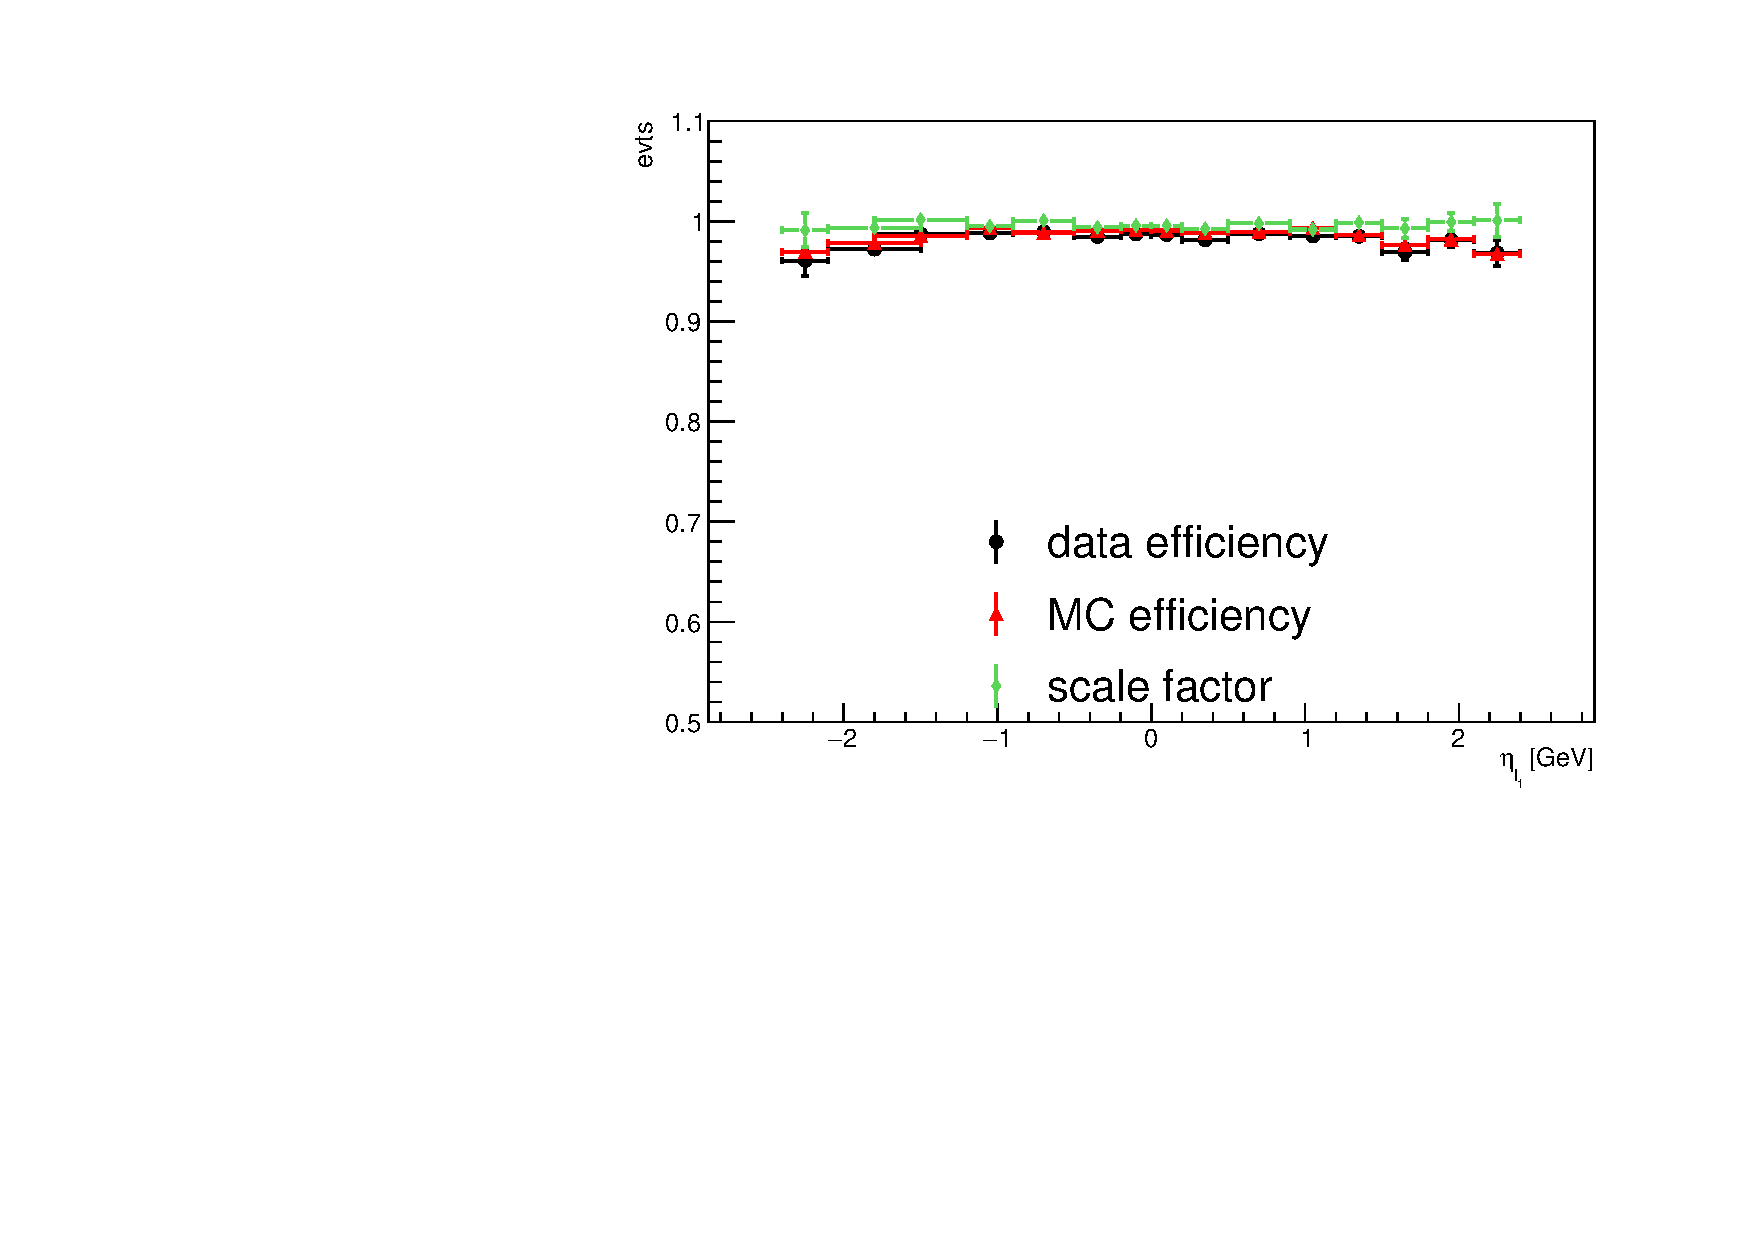
\includegraphics{Chapter1/Figures/MET/emu/leading_eta}}
    \resizebox{0.48 \textwidth}{!}{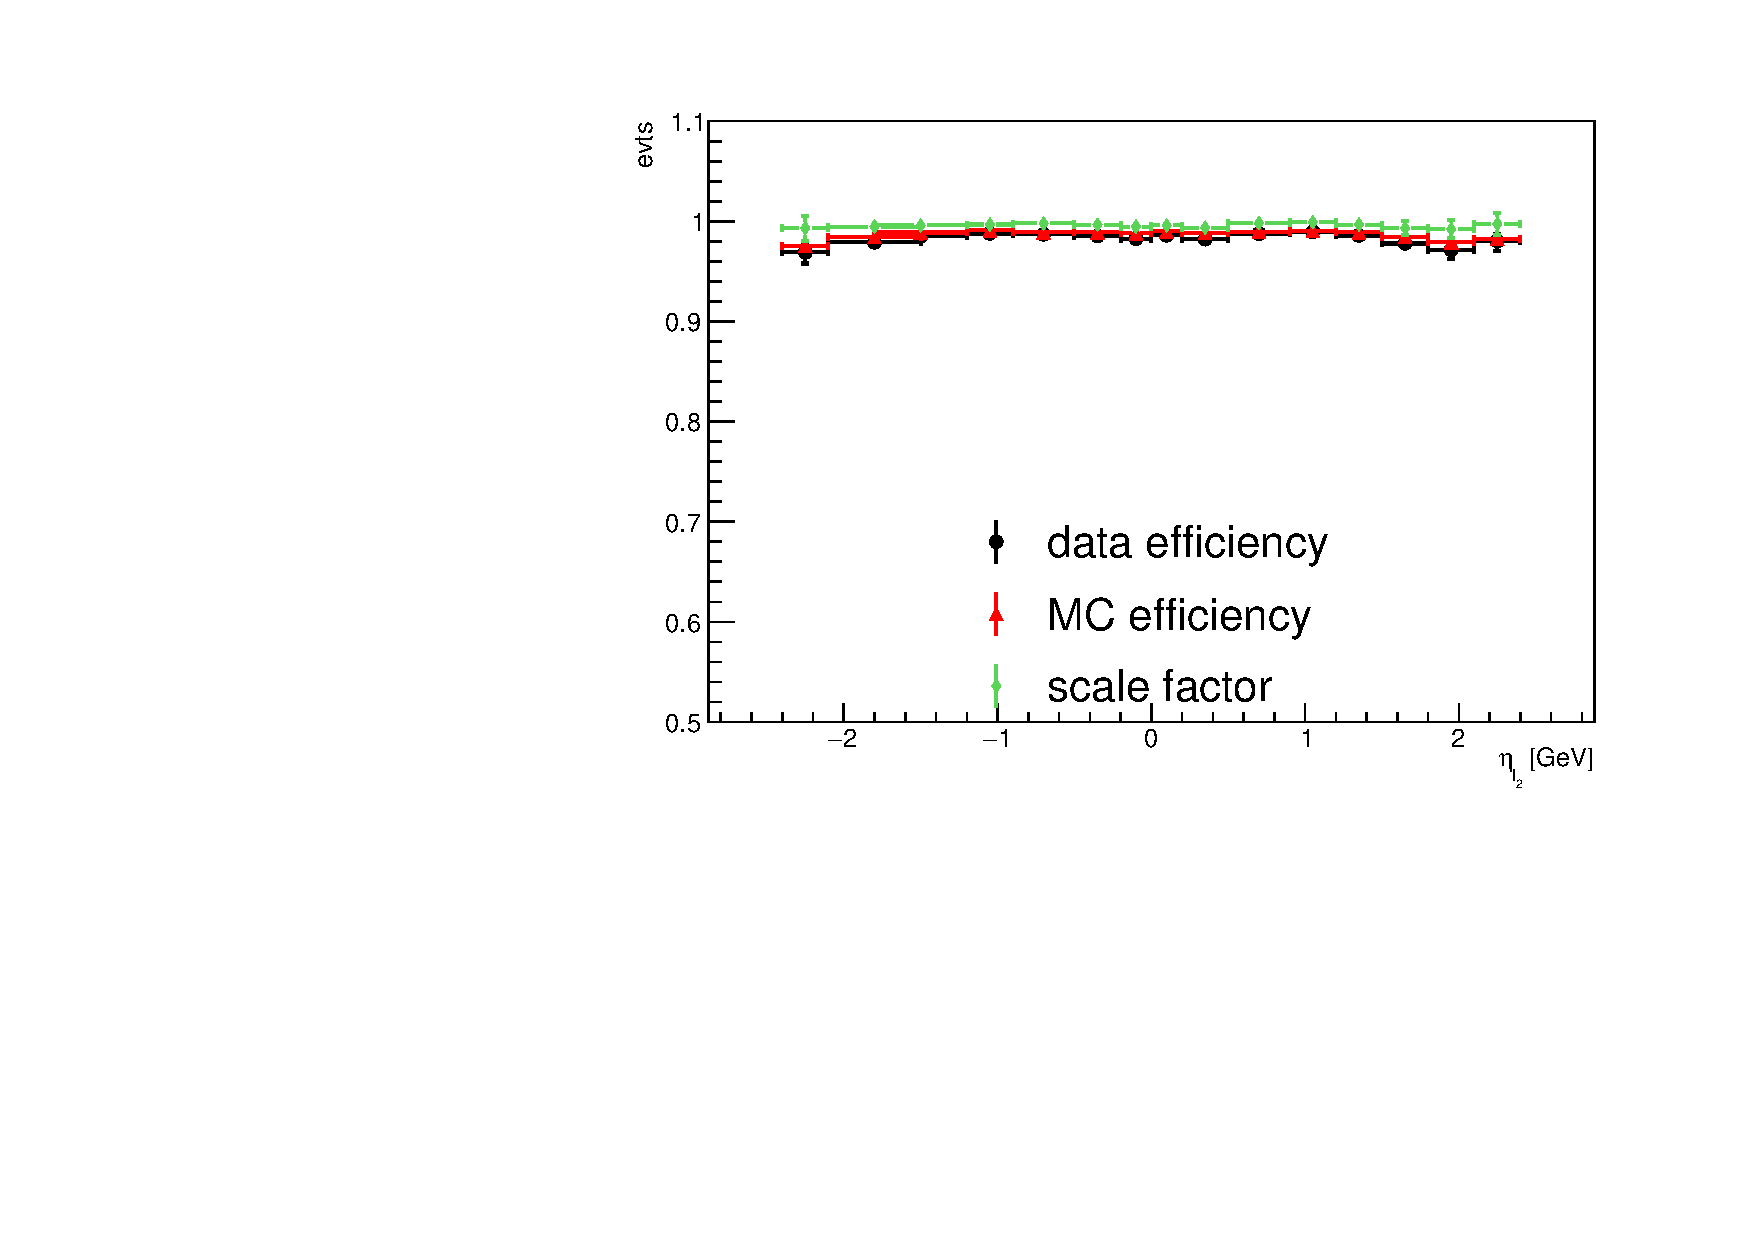
\includegraphics{Chapter1/Figures/MET/emu/seleading_eta}}
    \resizebox{0.48 \textwidth}{!}{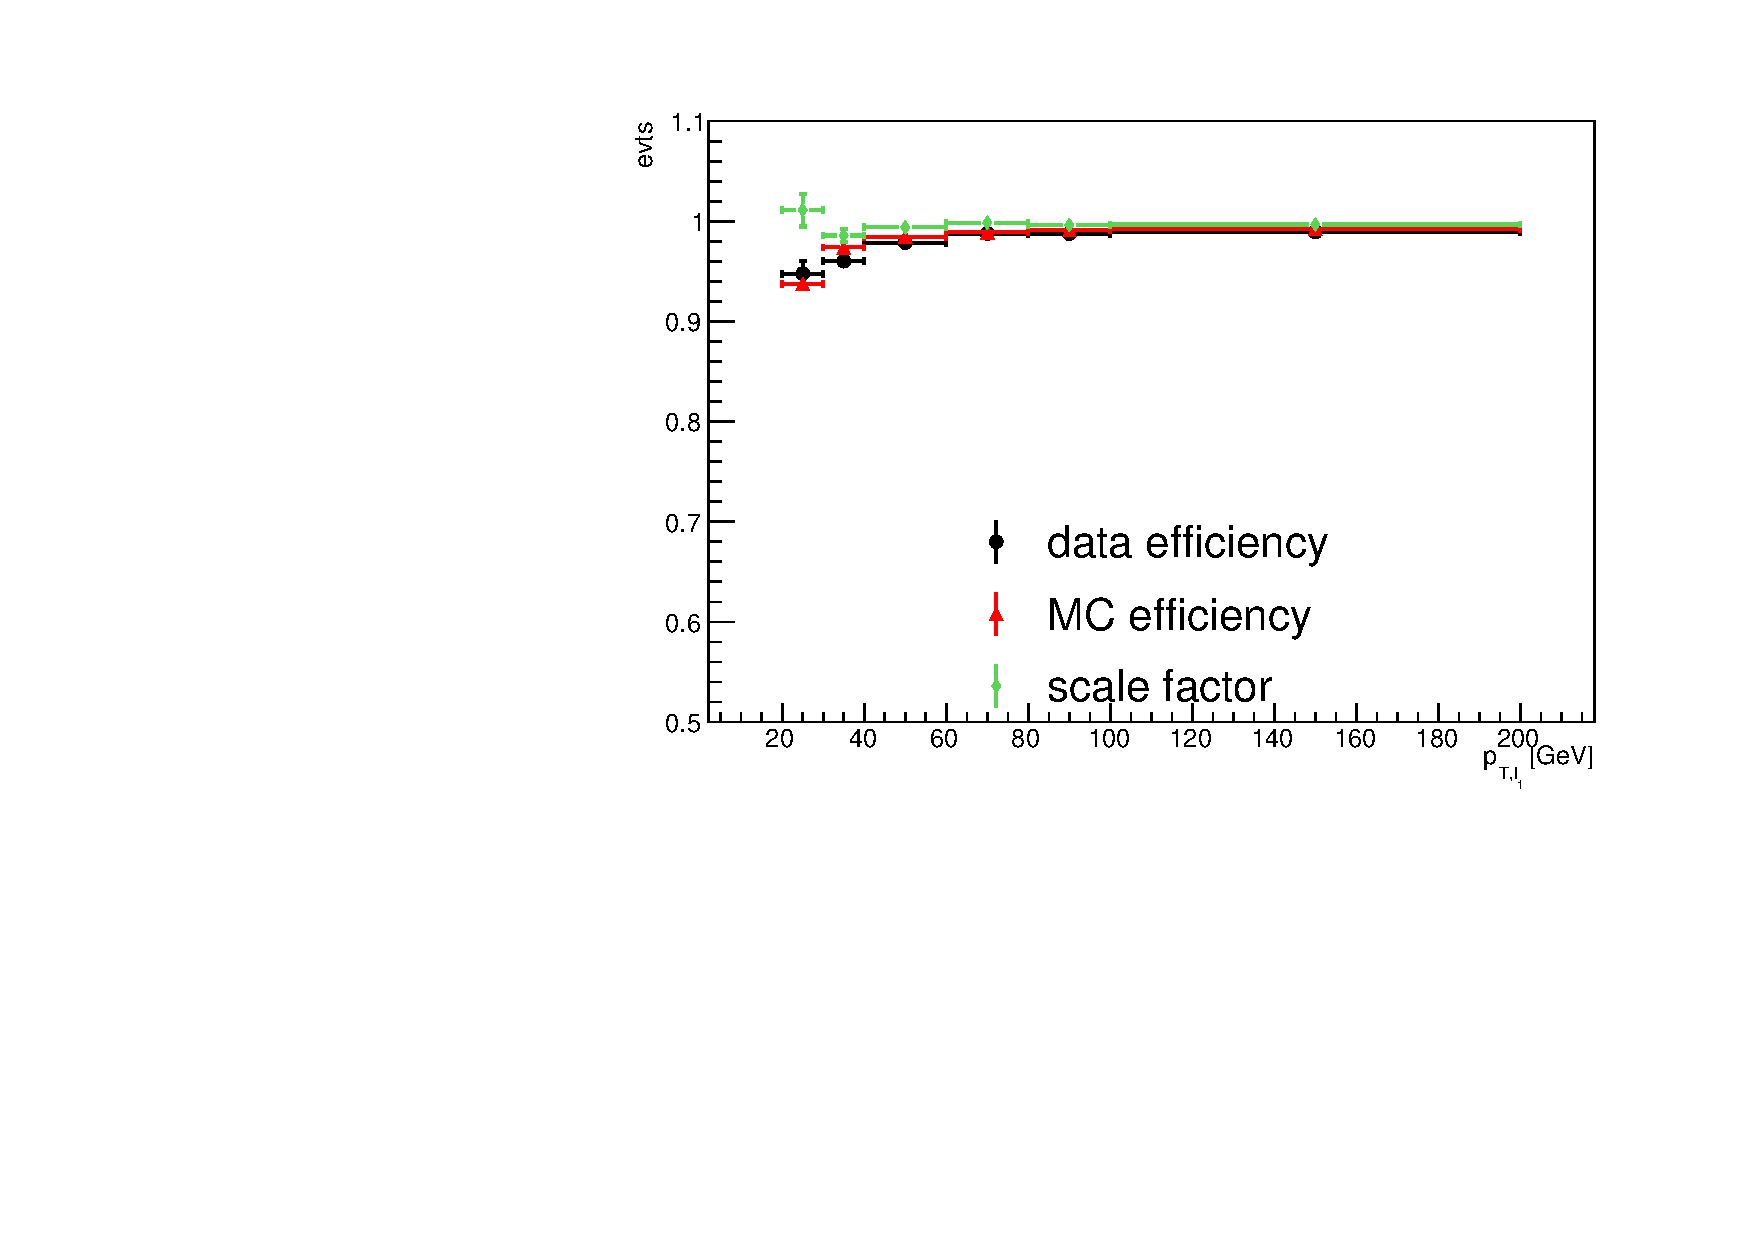
\includegraphics{Chapter1/Figures/MET/emu/leading_pt}}
    \resizebox{0.48 \textwidth}{!}{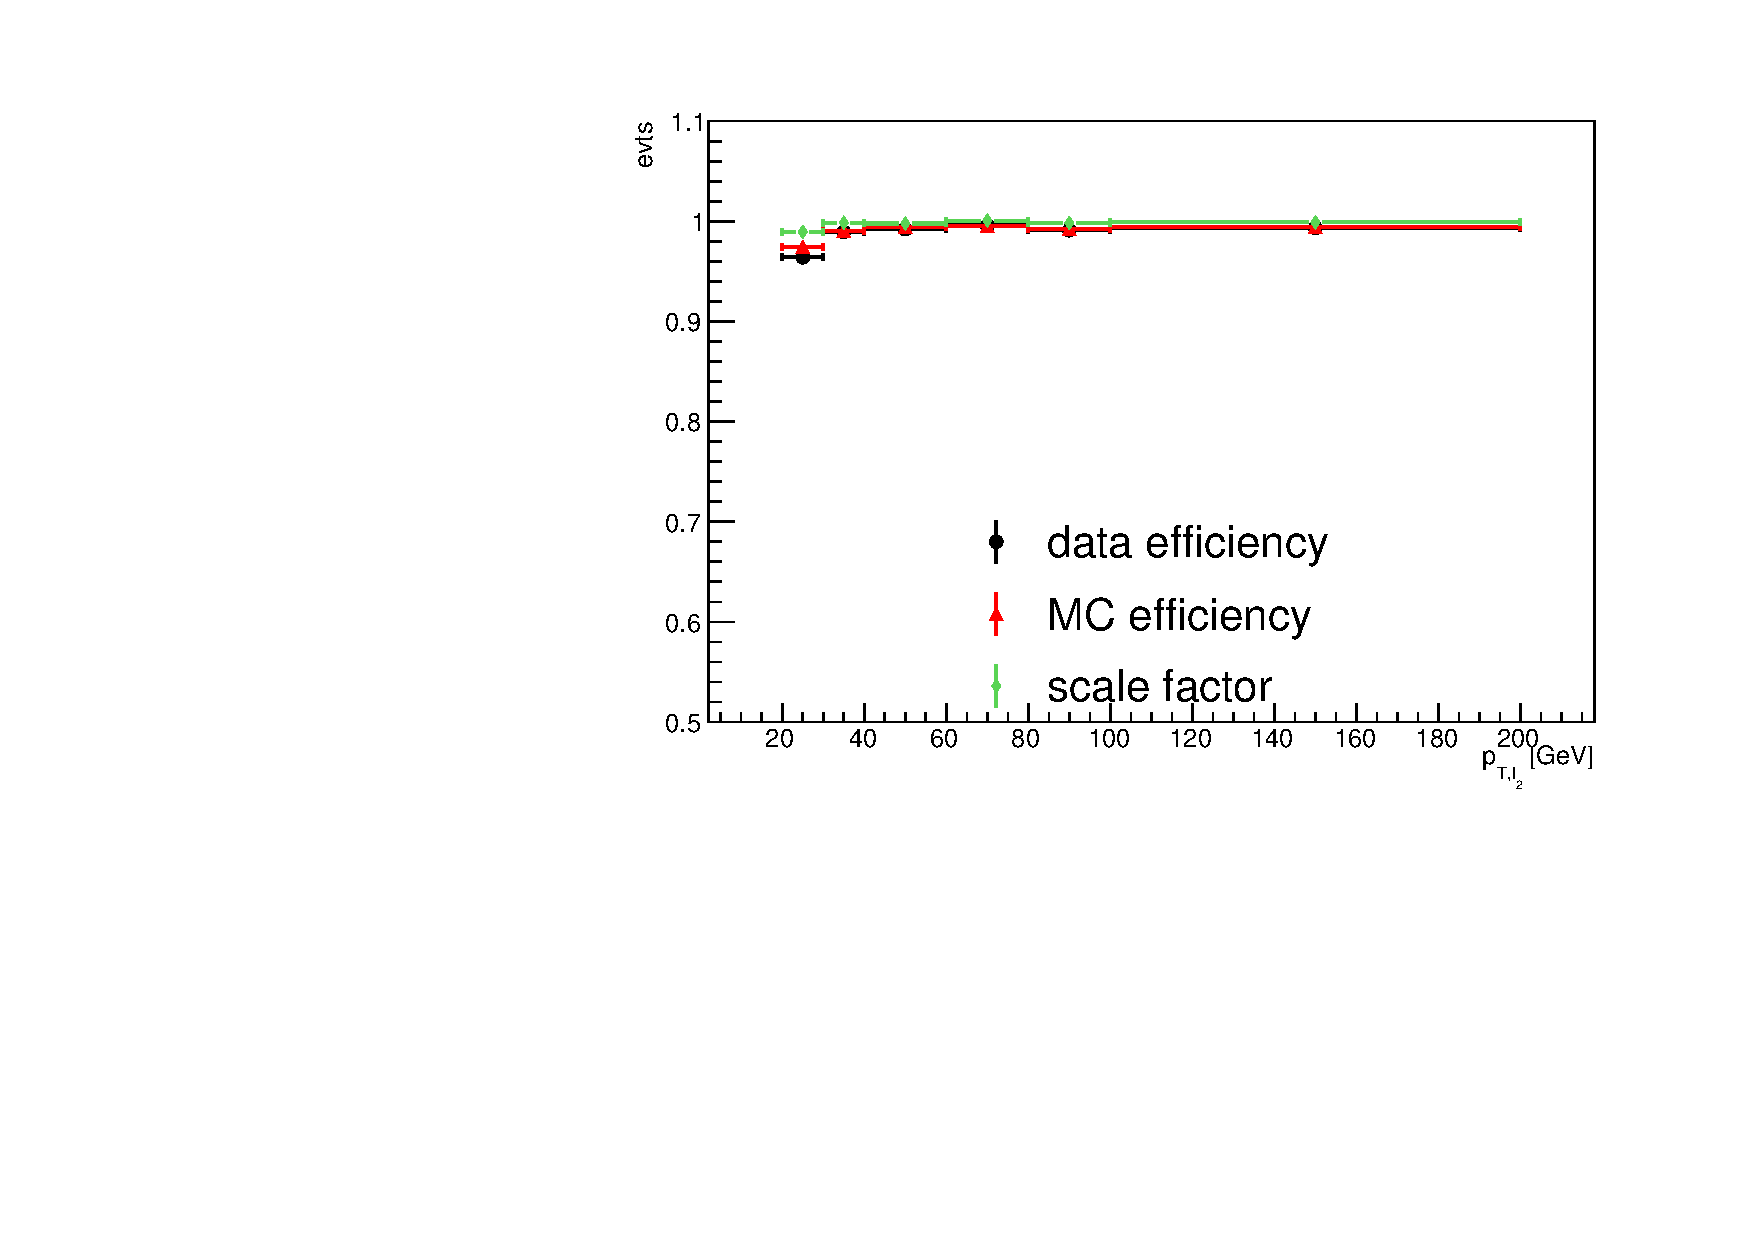
\includegraphics{Chapter1/Figures/MET/emu/seleading_pt}}
    \resizebox{0.48 \textwidth}{!}{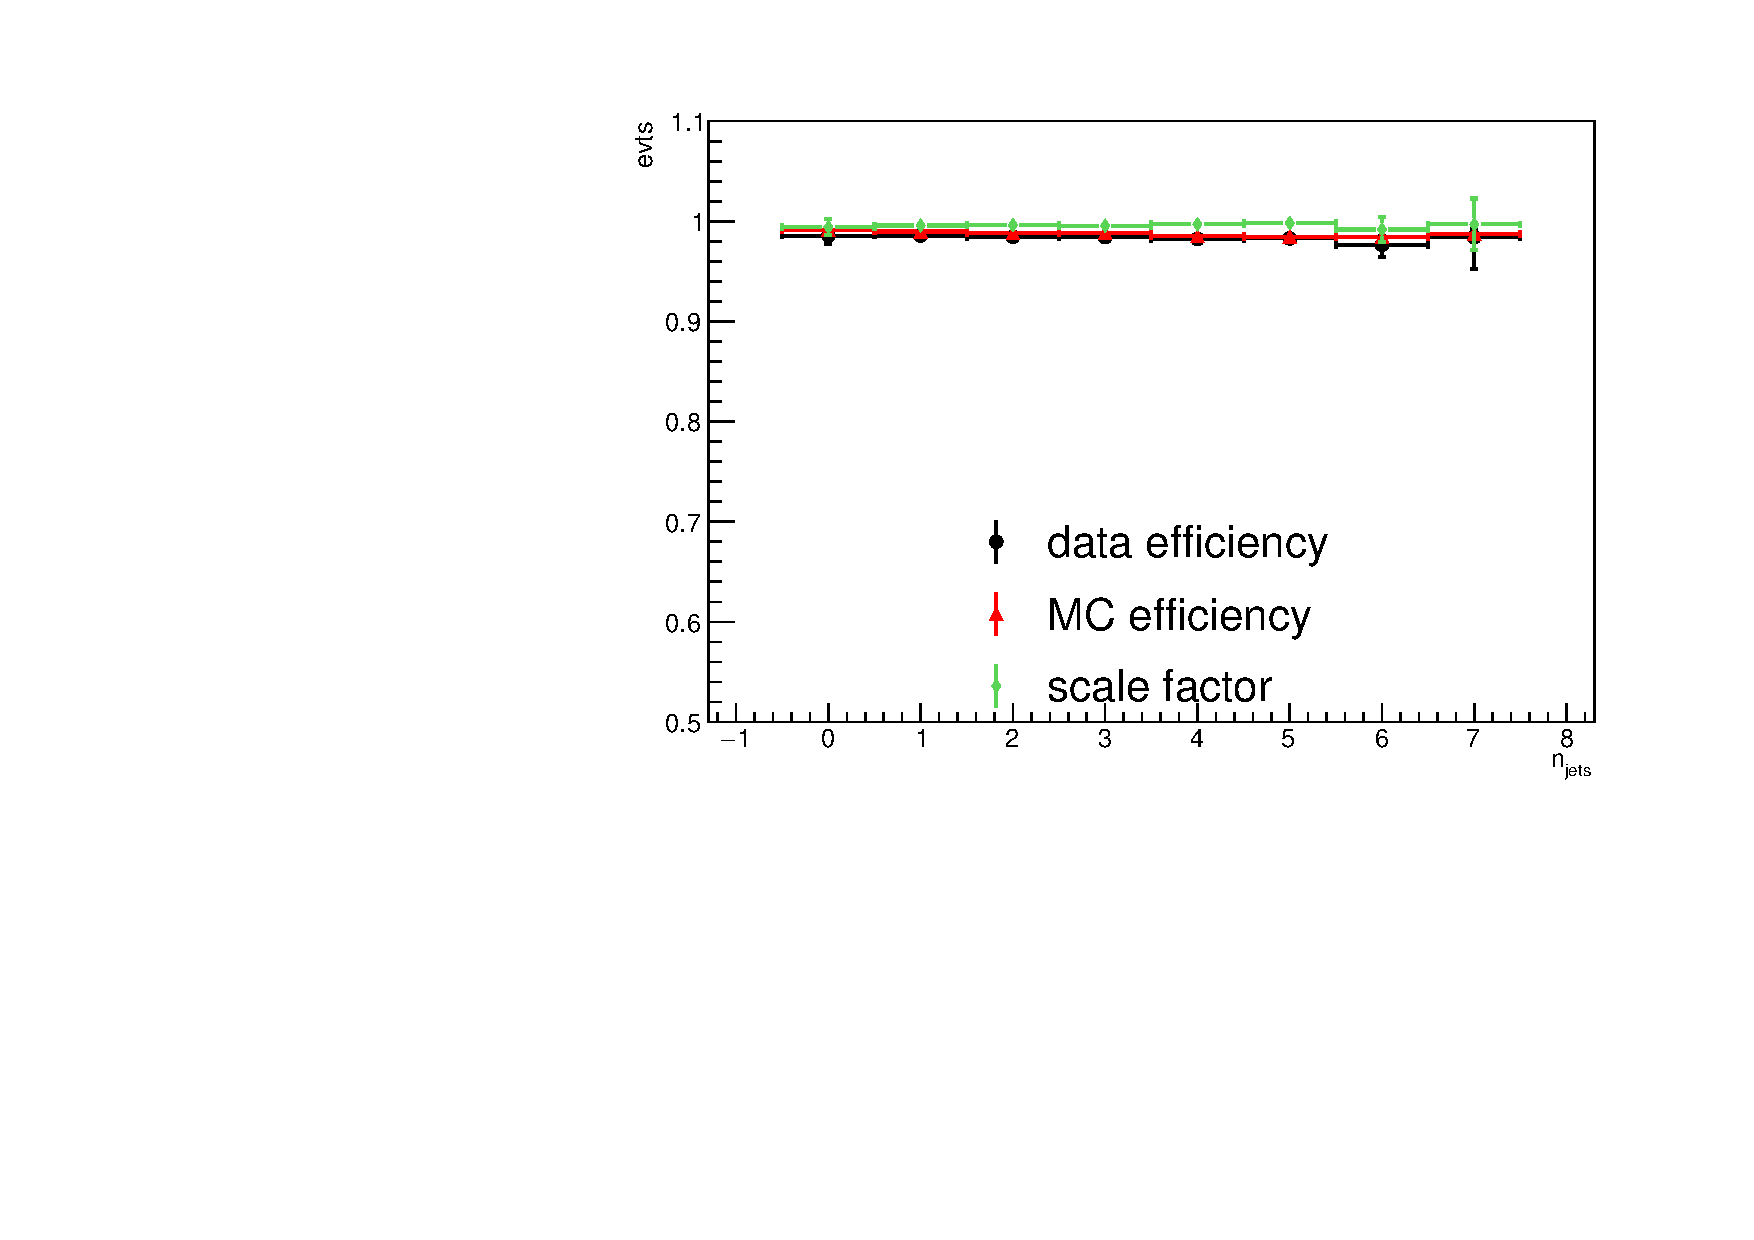
\includegraphics{Chapter1/Figures/MET/emu/jet_multi}}
    \resizebox{0.48 \textwidth}{!}{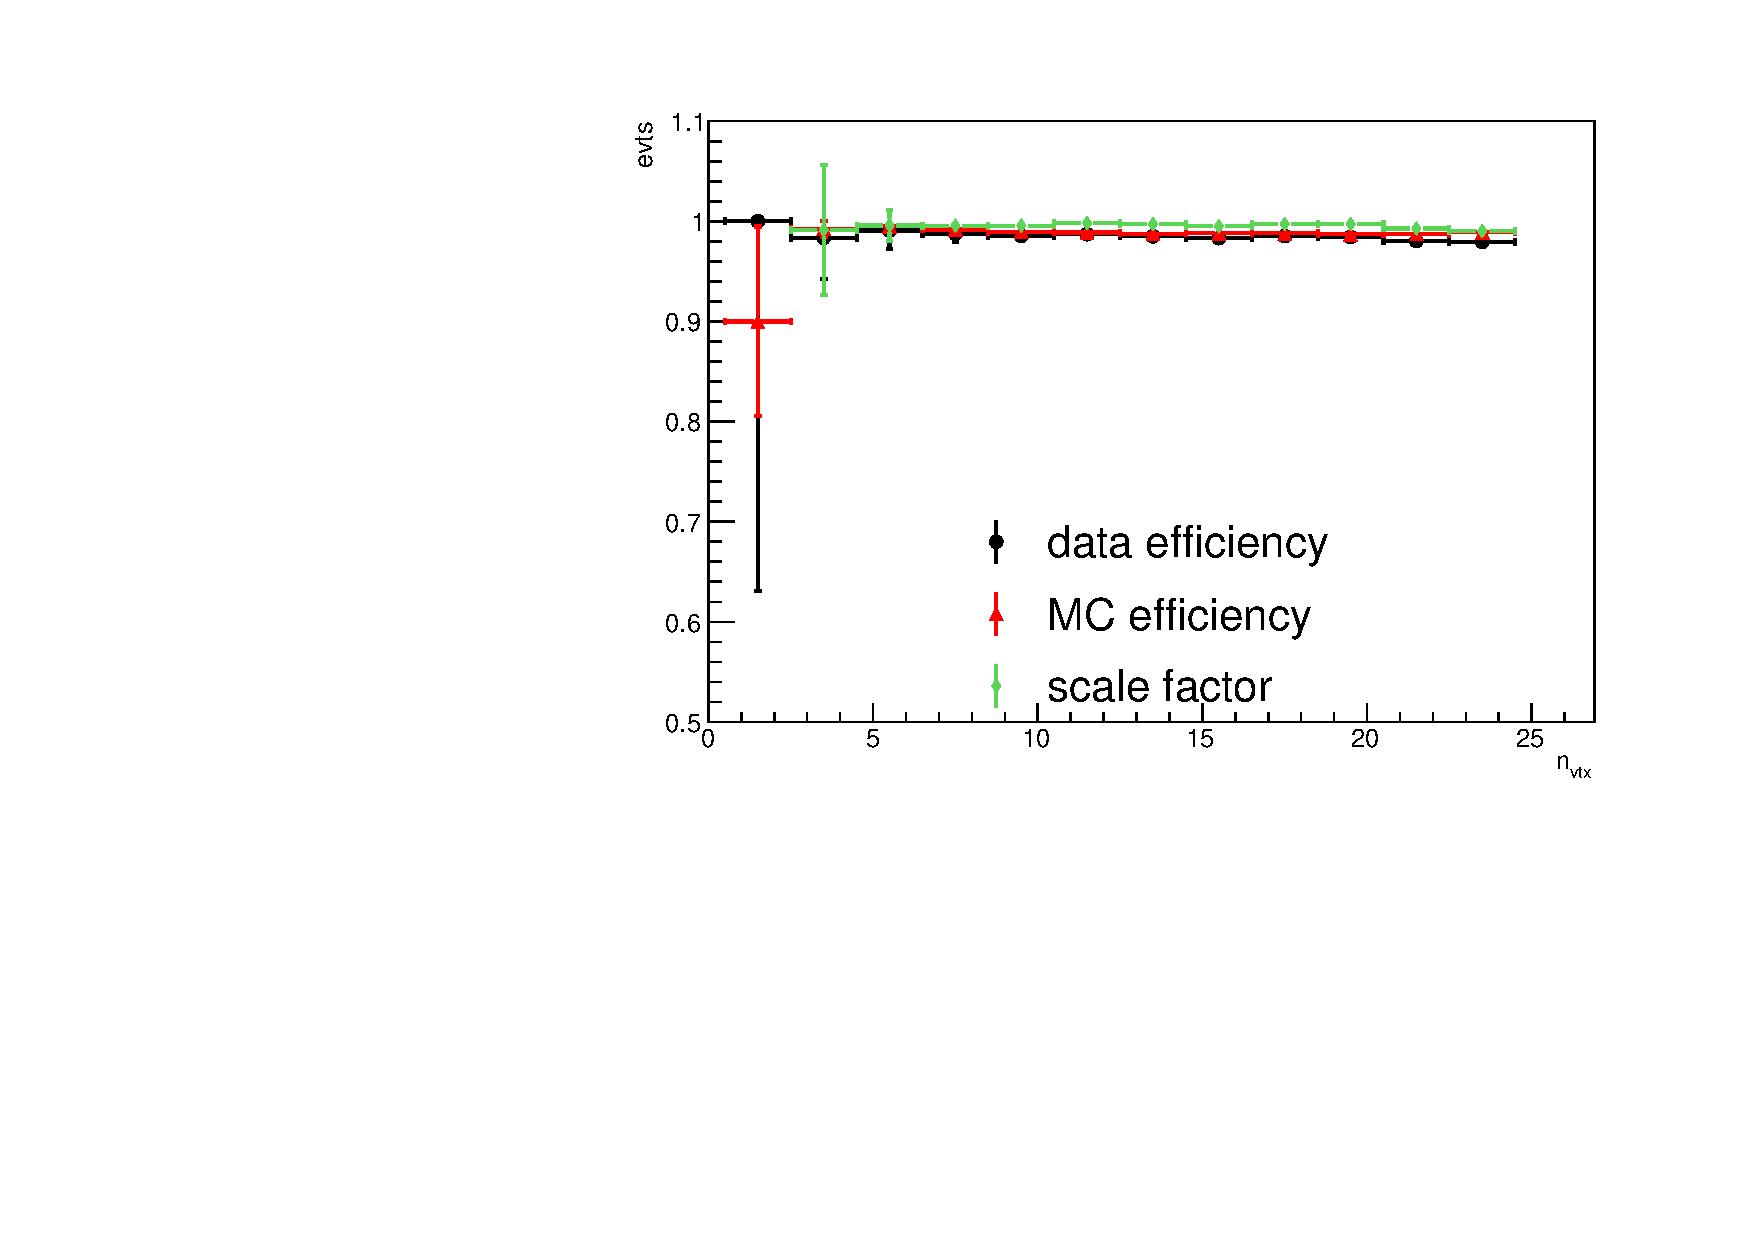
\includegraphics{Chapter1/Figures/MET/emu/vertex_multi}}  
      \caption{Efficiencies of the trigger selection in the \emu channel for simulation and data and the corresponding scale factor. The top row shows the efficiency depending on $\eta$ of the leading (left) and trailing (right) lepton. The middle row shows the effciency \pt of the leading (left) and trailing (right) lepton. The bottom rwo shows the efficiency depending on the jet multiplicity on the left and the vertex multiplicity on the right.
      The error bars denote statistical uncertainties. }  
      
    \label{fig:MET_emu}
  \end{center}
\end{figure}


%********************************** % Third Section  *************************************
\section{Where does it come from?}  %Section - 1.3 
\label{section1.3}
